% Options for packages loaded elsewhere
\PassOptionsToPackage{unicode}{hyperref}
\PassOptionsToPackage{hyphens}{url}
\documentclass[
]{book}
\usepackage{xcolor}
\usepackage{amsmath,amssymb}
\setcounter{secnumdepth}{5}
\usepackage{iftex}
\ifPDFTeX
  \usepackage[T1]{fontenc}
  \usepackage[utf8]{inputenc}
  \usepackage{textcomp} % provide euro and other symbols
\else % if luatex or xetex
  \usepackage{unicode-math} % this also loads fontspec
  \defaultfontfeatures{Scale=MatchLowercase}
  \defaultfontfeatures[\rmfamily]{Ligatures=TeX,Scale=1}
\fi
\usepackage{lmodern}
\ifPDFTeX\else
  % xetex/luatex font selection
\fi
% Use upquote if available, for straight quotes in verbatim environments
\IfFileExists{upquote.sty}{\usepackage{upquote}}{}
\IfFileExists{microtype.sty}{% use microtype if available
  \usepackage[]{microtype}
  \UseMicrotypeSet[protrusion]{basicmath} % disable protrusion for tt fonts
}{}
\makeatletter
\@ifundefined{KOMAClassName}{% if non-KOMA class
  \IfFileExists{parskip.sty}{%
    \usepackage{parskip}
  }{% else
    \setlength{\parindent}{0pt}
    \setlength{\parskip}{6pt plus 2pt minus 1pt}}
}{% if KOMA class
  \KOMAoptions{parskip=half}}
\makeatother
\usepackage{color}
\usepackage{fancyvrb}
\newcommand{\VerbBar}{|}
\newcommand{\VERB}{\Verb[commandchars=\\\{\}]}
\DefineVerbatimEnvironment{Highlighting}{Verbatim}{commandchars=\\\{\}}
% Add ',fontsize=\small' for more characters per line
\usepackage{framed}
\definecolor{shadecolor}{RGB}{248,248,248}
\newenvironment{Shaded}{\begin{snugshade}}{\end{snugshade}}
\newcommand{\AlertTok}[1]{\textcolor[rgb]{0.94,0.16,0.16}{#1}}
\newcommand{\AnnotationTok}[1]{\textcolor[rgb]{0.56,0.35,0.01}{\textbf{\textit{#1}}}}
\newcommand{\AttributeTok}[1]{\textcolor[rgb]{0.13,0.29,0.53}{#1}}
\newcommand{\BaseNTok}[1]{\textcolor[rgb]{0.00,0.00,0.81}{#1}}
\newcommand{\BuiltInTok}[1]{#1}
\newcommand{\CharTok}[1]{\textcolor[rgb]{0.31,0.60,0.02}{#1}}
\newcommand{\CommentTok}[1]{\textcolor[rgb]{0.56,0.35,0.01}{\textit{#1}}}
\newcommand{\CommentVarTok}[1]{\textcolor[rgb]{0.56,0.35,0.01}{\textbf{\textit{#1}}}}
\newcommand{\ConstantTok}[1]{\textcolor[rgb]{0.56,0.35,0.01}{#1}}
\newcommand{\ControlFlowTok}[1]{\textcolor[rgb]{0.13,0.29,0.53}{\textbf{#1}}}
\newcommand{\DataTypeTok}[1]{\textcolor[rgb]{0.13,0.29,0.53}{#1}}
\newcommand{\DecValTok}[1]{\textcolor[rgb]{0.00,0.00,0.81}{#1}}
\newcommand{\DocumentationTok}[1]{\textcolor[rgb]{0.56,0.35,0.01}{\textbf{\textit{#1}}}}
\newcommand{\ErrorTok}[1]{\textcolor[rgb]{0.64,0.00,0.00}{\textbf{#1}}}
\newcommand{\ExtensionTok}[1]{#1}
\newcommand{\FloatTok}[1]{\textcolor[rgb]{0.00,0.00,0.81}{#1}}
\newcommand{\FunctionTok}[1]{\textcolor[rgb]{0.13,0.29,0.53}{\textbf{#1}}}
\newcommand{\ImportTok}[1]{#1}
\newcommand{\InformationTok}[1]{\textcolor[rgb]{0.56,0.35,0.01}{\textbf{\textit{#1}}}}
\newcommand{\KeywordTok}[1]{\textcolor[rgb]{0.13,0.29,0.53}{\textbf{#1}}}
\newcommand{\NormalTok}[1]{#1}
\newcommand{\OperatorTok}[1]{\textcolor[rgb]{0.81,0.36,0.00}{\textbf{#1}}}
\newcommand{\OtherTok}[1]{\textcolor[rgb]{0.56,0.35,0.01}{#1}}
\newcommand{\PreprocessorTok}[1]{\textcolor[rgb]{0.56,0.35,0.01}{\textit{#1}}}
\newcommand{\RegionMarkerTok}[1]{#1}
\newcommand{\SpecialCharTok}[1]{\textcolor[rgb]{0.81,0.36,0.00}{\textbf{#1}}}
\newcommand{\SpecialStringTok}[1]{\textcolor[rgb]{0.31,0.60,0.02}{#1}}
\newcommand{\StringTok}[1]{\textcolor[rgb]{0.31,0.60,0.02}{#1}}
\newcommand{\VariableTok}[1]{\textcolor[rgb]{0.00,0.00,0.00}{#1}}
\newcommand{\VerbatimStringTok}[1]{\textcolor[rgb]{0.31,0.60,0.02}{#1}}
\newcommand{\WarningTok}[1]{\textcolor[rgb]{0.56,0.35,0.01}{\textbf{\textit{#1}}}}
\usepackage{longtable,booktabs,array}
\usepackage{calc} % for calculating minipage widths
% Correct order of tables after \paragraph or \subparagraph
\usepackage{etoolbox}
\makeatletter
\patchcmd\longtable{\par}{\if@noskipsec\mbox{}\fi\par}{}{}
\makeatother
% Allow footnotes in longtable head/foot
\IfFileExists{footnotehyper.sty}{\usepackage{footnotehyper}}{\usepackage{footnote}}
\makesavenoteenv{longtable}
\usepackage{graphicx}
\makeatletter
\newsavebox\pandoc@box
\newcommand*\pandocbounded[1]{% scales image to fit in text height/width
  \sbox\pandoc@box{#1}%
  \Gscale@div\@tempa{\textheight}{\dimexpr\ht\pandoc@box+\dp\pandoc@box\relax}%
  \Gscale@div\@tempb{\linewidth}{\wd\pandoc@box}%
  \ifdim\@tempb\p@<\@tempa\p@\let\@tempa\@tempb\fi% select the smaller of both
  \ifdim\@tempa\p@<\p@\scalebox{\@tempa}{\usebox\pandoc@box}%
  \else\usebox{\pandoc@box}%
  \fi%
}
% Set default figure placement to htbp
\def\fps@figure{htbp}
\makeatother
\setlength{\emergencystretch}{3em} % prevent overfull lines
\providecommand{\tightlist}{%
  \setlength{\itemsep}{0pt}\setlength{\parskip}{0pt}}
\usepackage[]{natbib}
\bibliographystyle{plainnat}
\usepackage{bookmark}
\IfFileExists{xurl.sty}{\usepackage{xurl}}{} % add URL line breaks if available
\urlstyle{same}
\hypersetup{
  pdftitle={Machine Learning for Biostatistics},
  pdfauthor={Jaroslaw Harezlak \& Armando Teixeira-Pinto},
  hidelinks,
  pdfcreator={LaTeX via pandoc}}

\title{Machine Learning for Biostatistics}
\usepackage{etoolbox}
\makeatletter
\providecommand{\subtitle}[1]{% add subtitle to \maketitle
  \apptocmd{\@title}{\par {\large #1 \par}}{}{}
}
\makeatother
\subtitle{Module 5}
\author{Jaroslaw Harezlak \& Armando Teixeira-Pinto}
\date{2025-08-08}

\begin{document}
\maketitle

{
\setcounter{tocdepth}{1}
\tableofcontents
}
\chapter*{Beyond Linearity}\label{beyond-linearity}
\addcontentsline{toc}{chapter}{Beyond Linearity}

\section*{Introduction}\label{introduction}
\addcontentsline{toc}{section}{Introduction}

This module will cover methods to explore non-linear effects of numerical
predictors on the outcome.

By the end of this module you should be able to:

\begin{enumerate}
\def\labelenumi{\arabic{enumi}.}
\tightlist
\item
  Identify approaches to model non-linear effects
\item
  Implement linear and polynomial piecewise regression
\item
  Understand the difference between polynomial splines, b-splines and natural
  splines
\item
  Fit a GLM with different splines
\item
  Use smoothing splines to approximate non-linear effects
\item
  Integrate smoothing splines in modeling strategies using generalised additive models
\end{enumerate}

\section*{Dataset used in the examples}\label{dataset-used-in-the-examples}
\addcontentsline{toc}{section}{Dataset used in the examples}

The dataset \textbf{triceps} is available in the \texttt{MultiKink} package.
You may \texttt{install.packages("MultiKink")}, load the library (\texttt{library(MultiKink)})
and then run \texttt{data("triceps")}.

The data are derived from an anthropometric study of 892 females under 50 years
in three Gambian villages in West Africa. There are 892 observations
on the following 3 variables:

\begin{itemize}
\tightlist
\item
  age - Age of respondents.
\item
  lntriceps - Log of the triceps skinfold thickness.
\item
  triceps - Triceps skinfold thickness.
\end{itemize}

\begin{center}\rule{0.5\linewidth}{0.5pt}\end{center}

The data \href{https://www.dropbox.com/s/cwkw3p91zyizcqz/SA_heart.csv?dl=1}{SA\_heart.csv}
is retrospective sample of males in a heart-disease high-risk region of the
Western Cape, South Africa. There are roughly two controls per case of CHD.

Many of the CHD positive men have undergone blood pressure
reduction treatment and other programs to reduce their risk factors after
their CHD event. In some cases the measurements were made after these
treatments. These data are taken from a larger dataset,
described in Rousseauw et al, 1983, South African Medical Journal.

The data contains 462 observations on the following 10 variables.

\begin{itemize}
\tightlist
\item
  sbp - systolic blood pressure
\item
  tobacco - cumulative tobacco (kg)
\item
  ldl - low density lipoprotein cholesterol
\item
  adiposity - a numeric vector
\item
  famhist - family history of heart disease, a factor
  with levels Absent Present
\item
  typea - type-A behavior
\item
  obesity - a numeric vector
\item
  alcohol - current alcohol consumption
\item
  age - age at onset
\item
  chd- response, coronary heart disease (1 - chd, 0 - no chd)
\end{itemize}

\section*{Slides from the videos}\label{slides-from-the-videos}
\addcontentsline{toc}{section}{Slides from the videos}

You can download the slides used in the videos form Beyond Linearity:

\href{https://www.dropbox.com/s/att3vxk1wr9rcuu/Module-5-Beyond-Linearity_2020.pdf?dl=1}{Slides}

\chapter{Polynomial Regression}\label{polynomial-regression}

\section{Introduction}\label{PR1}

The extension of the linear models \(y=\beta_0 + \beta_1x + \varepsilon\) to
include higher degree polynomial terms \(x^2\), \(x^3\), \ldots, \(x^p\) is
straightforward. Each additional term can be viewed as another predictor in
the regression equation:

\(y=\beta_0 + \beta_1x + \beta_2x^2 + \dots + \beta_px^p + \varepsilon\)

This allows the fit of more flexible models representing the association between the
outcome and some continuous predictors.

\pandocbounded{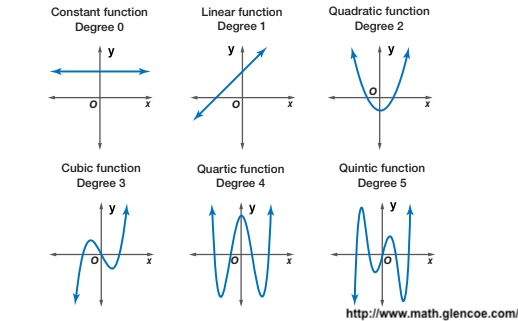
\includegraphics[keepaspectratio]{PolynomialFunctionsGraph.PNG}}

However, in practice, we hardly go beyond the degree 3. If the association
between the outcome and predictor is highly non-linear, than it is preferable
to use the methods that we will discuss in the next sections.

\section{Readings}\label{PR2}

Read the following chapters of \emph{An introduction to statistical learning}:

\begin{itemize}
\tightlist
\item
  7.1 Polynomial Regression
\end{itemize}

\section{Practice session}\label{PR3}

\subsection*{Task 1 - Fit a cubic model}\label{task-1---fit-a-cubic-model}
\addcontentsline{toc}{subsection}{Task 1 - Fit a cubic model}

The dataset \textbf{triceps} is available in the \texttt{MultiKink} package.

The data contains the measurement of the triceps skin fold of 892 females
(variable \emph{triceps}) and we want to model its association with \textbf{age}.

First, we will load the data

\begin{Shaded}
\begin{Highlighting}[]
\CommentTok{\#libraries that we will need}
\CommentTok{\#install.packages("MultiKink")  }
\FunctionTok{library}\NormalTok{(MultiKink) }\CommentTok{\#for the data}
\FunctionTok{library}\NormalTok{(ggplot2)   }\CommentTok{\#for the plots}
\end{Highlighting}
\end{Shaded}

\begin{verbatim}
## Warning: package 'ggplot2' was built under R version 4.3.3
\end{verbatim}

\begin{Shaded}
\begin{Highlighting}[]
\FunctionTok{set.seed}\NormalTok{(}\DecValTok{1974}\NormalTok{)     }\CommentTok{\#fix the random generator seed }

\FunctionTok{data}\NormalTok{(}\StringTok{"triceps"}\NormalTok{)   }\CommentTok{\#load the dataset triceps}
                  \CommentTok{\#notice that the variable of interest}
                  \CommentTok{\#it is also called triceps. Don\textquotesingle{}t get }
                  \CommentTok{\#confused!}
\end{Highlighting}
\end{Shaded}

And plot the scatter for \textbf{triceps} and \textbf{age}

\begin{Shaded}
\begin{Highlighting}[]
 \CommentTok{\#simple scatter}
  \CommentTok{\#we can store the scatter in an object }
  \CommentTok{\#to use it later}
\NormalTok{ tri.age.plot }\OtherTok{\textless{}{-}} \FunctionTok{ggplot}\NormalTok{(triceps, }\FunctionTok{aes}\NormalTok{(}\AttributeTok{x=}\NormalTok{age, }\AttributeTok{y=}\NormalTok{triceps)) }\SpecialCharTok{+}
                 \FunctionTok{geom\_point}\NormalTok{(}\AttributeTok{alpha=}\FloatTok{0.55}\NormalTok{, }\AttributeTok{color=}\StringTok{"black"}\NormalTok{) }\SpecialCharTok{+} 
                 \FunctionTok{theme\_minimal}\NormalTok{() }
\NormalTok{ tri.age.plot}
\end{Highlighting}
\end{Shaded}

\pandocbounded{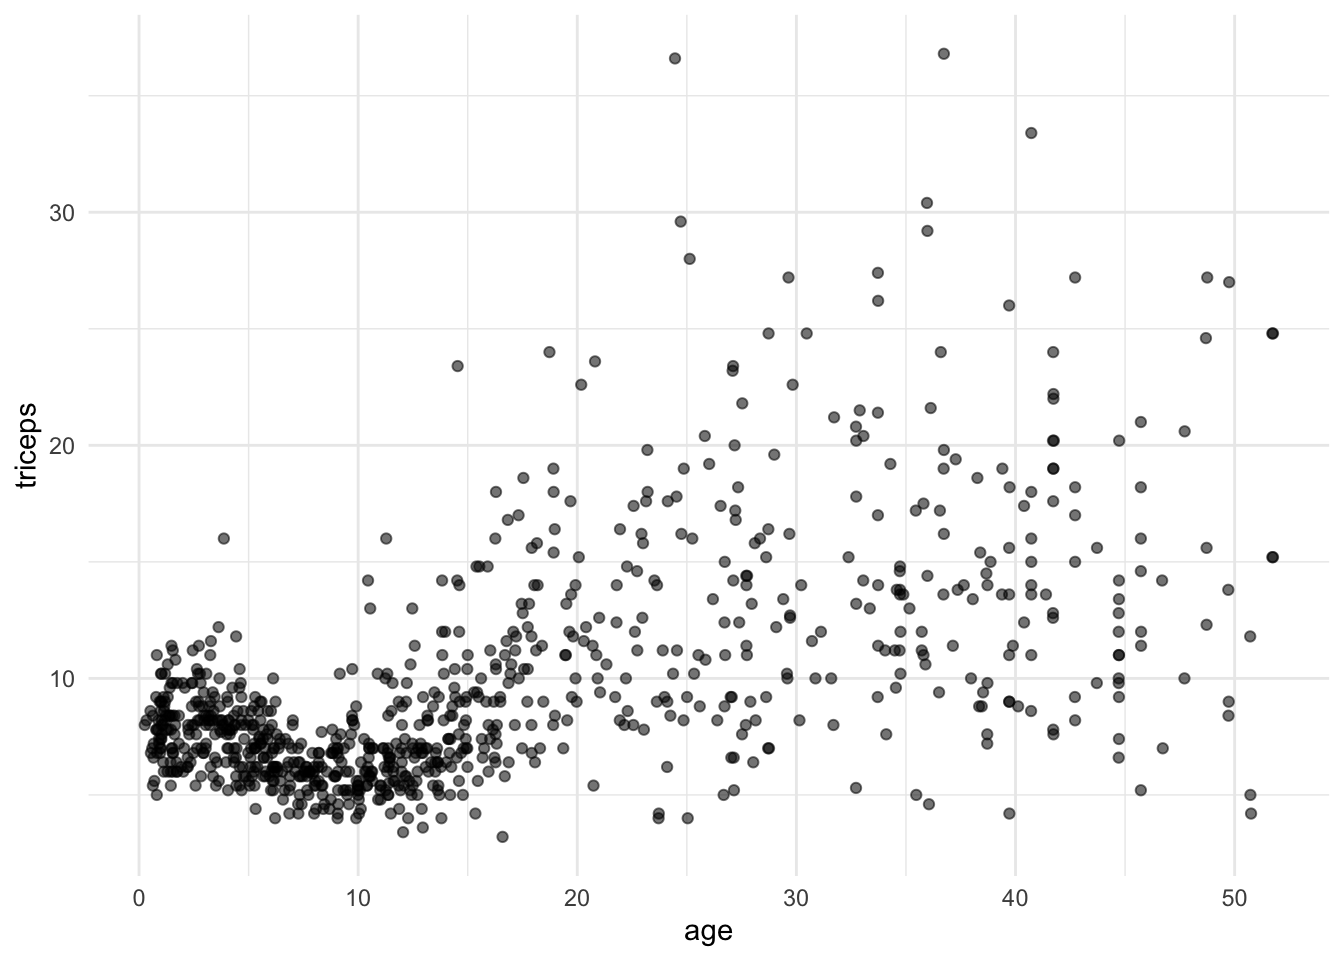
\includegraphics[keepaspectratio]{_main_files/figure-latex/plotagetric0-1.pdf}}

To fit a cubic model we can write all the terms using the \texttt{I()} function to
evaluate \(x^2\) and \(x^3\), otherwise R will not use the quadratic and cubic terms:

\begin{Shaded}
\begin{Highlighting}[]
\NormalTok{model.cubic }\OtherTok{\textless{}{-}} \FunctionTok{lm}\NormalTok{(triceps}\SpecialCharTok{\textasciitilde{}}\NormalTok{age }\SpecialCharTok{+} \FunctionTok{I}\NormalTok{(age}\SpecialCharTok{\^{}}\DecValTok{2}\NormalTok{) }\SpecialCharTok{+} \FunctionTok{I}\NormalTok{(age}\SpecialCharTok{\^{}}\DecValTok{3}\NormalTok{),}
                  \AttributeTok{data=}\NormalTok{triceps)}
\FunctionTok{summary}\NormalTok{(model.cubic)}
\end{Highlighting}
\end{Shaded}

\begin{verbatim}
## 
## Call:
## lm(formula = triceps ~ age + I(age^2) + I(age^3), data = triceps)
## 
## Residuals:
##      Min       1Q   Median       3Q      Max 
## -11.5832  -1.9284  -0.5415   1.3283  24.4440 
## 
## Coefficients:
##               Estimate Std. Error t value Pr(>|t|)    
## (Intercept)  8.004e+00  3.831e-01  20.893  < 2e-16 ***
## age         -3.157e-01  7.721e-02  -4.089 4.73e-05 ***
## I(age^2)     3.101e-02  3.964e-03   7.824 1.45e-14 ***
## I(age^3)    -4.566e-04  5.612e-05  -8.135 1.38e-15 ***
## ---
## Signif. codes:  0 '***' 0.001 '**' 0.01 '*' 0.05 '.' 0.1 ' ' 1
## 
## Residual standard error: 3.868 on 888 degrees of freedom
## Multiple R-squared:  0.3836, Adjusted R-squared:  0.3815 
## F-statistic: 184.2 on 3 and 888 DF,  p-value: < 2.2e-16
\end{verbatim}

Another option is to use the \texttt{poly()} function. Note, however, that the this
function fits a \textbf{linear transformation} of the terms \(x, x^2,x^3\). This is
for numerical stability given that those three terms will be highly correlated.
Thus, the regression coefficients will not be the same but the model is just
a reparameterisation of the one above and its predictions are exactly the same.

\begin{Shaded}
\begin{Highlighting}[]
\NormalTok{model.cubic.poly }\OtherTok{\textless{}{-}} \FunctionTok{lm}\NormalTok{(triceps}\SpecialCharTok{\textasciitilde{}}\FunctionTok{poly}\NormalTok{(age,}\DecValTok{3}\NormalTok{),}
                       \AttributeTok{data=}\NormalTok{triceps)}
\FunctionTok{summary}\NormalTok{(model.cubic.poly)}
\end{Highlighting}
\end{Shaded}

\begin{verbatim}
## 
## Call:
## lm(formula = triceps ~ poly(age, 3), data = triceps)
## 
## Residuals:
##      Min       1Q   Median       3Q      Max 
## -11.5832  -1.9284  -0.5415   1.3283  24.4440 
## 
## Coefficients:
##               Estimate Std. Error t value Pr(>|t|)    
## (Intercept)     9.7024     0.1295  74.911  < 2e-16 ***
## poly(age, 3)1  85.2594     3.8682  22.041  < 2e-16 ***
## poly(age, 3)2  -3.1638     3.8682  -0.818    0.414    
## poly(age, 3)3 -31.4683     3.8682  -8.135 1.38e-15 ***
## ---
## Signif. codes:  0 '***' 0.001 '**' 0.01 '*' 0.05 '.' 0.1 ' ' 1
## 
## Residual standard error: 3.868 on 888 degrees of freedom
## Multiple R-squared:  0.3836, Adjusted R-squared:  0.3815 
## F-statistic: 184.2 on 3 and 888 DF,  p-value: < 2.2e-16
\end{verbatim}

If you look at the predictions of both model, the results are exactly the same

\begin{Shaded}
\begin{Highlighting}[]
 \FunctionTok{plot}\NormalTok{(}\FunctionTok{predict}\NormalTok{(model.cubic.poly), }\FunctionTok{predict}\NormalTok{(model.cubic))}
\end{Highlighting}
\end{Shaded}

\pandocbounded{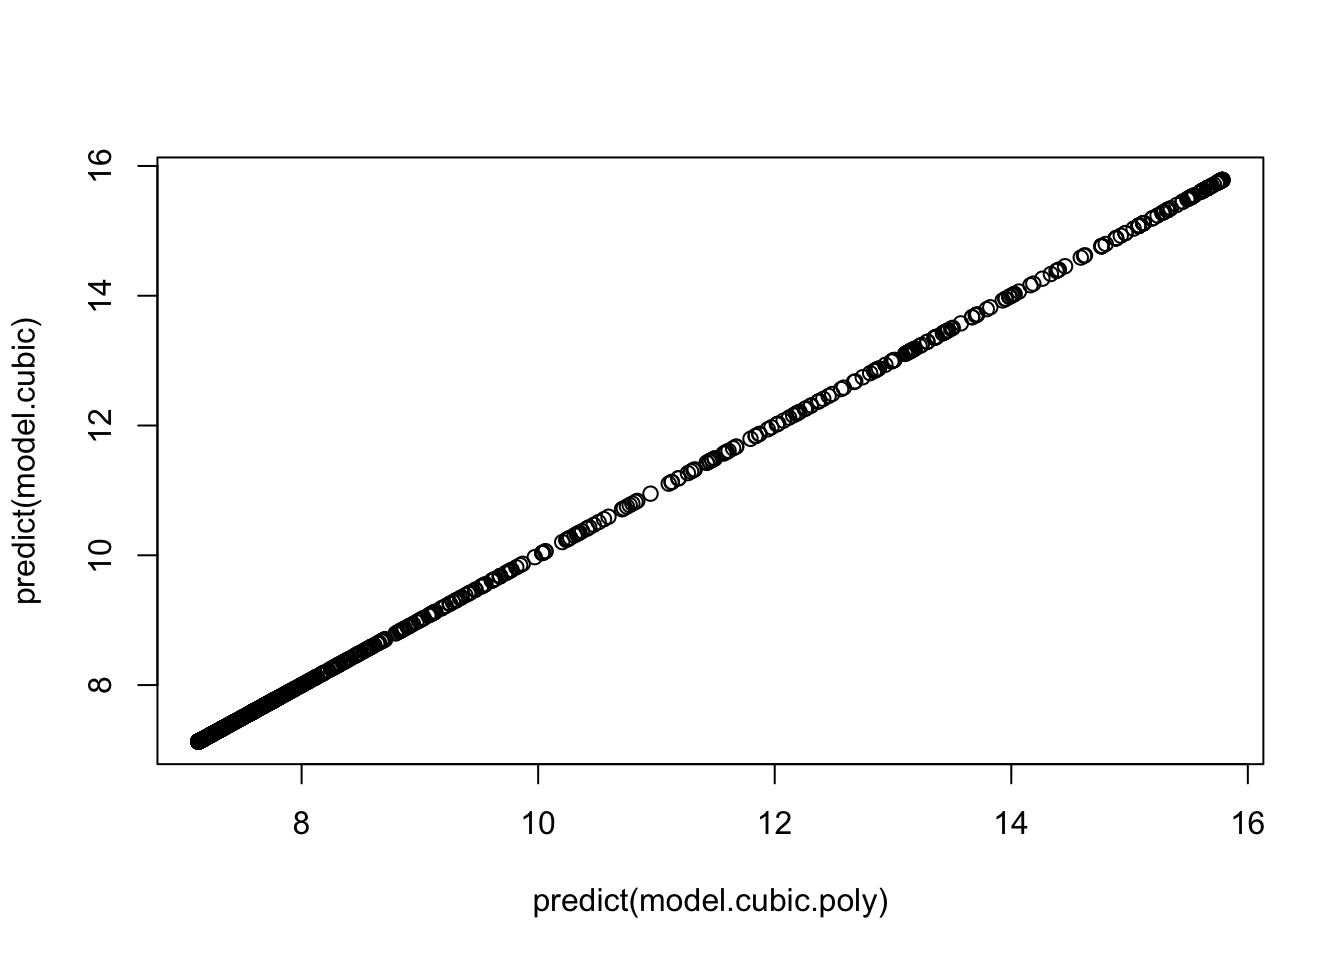
\includegraphics[keepaspectratio]{_main_files/figure-latex/pr.cub-1.pdf}}

We can also fit and plot the cubic model using \texttt{ggplot}. We will use the initial
scatter plot an add the fitted curve

\begin{Shaded}
\begin{Highlighting}[]
 \CommentTok{\#plots}
\NormalTok{ tri.age.plot }\SpecialCharTok{+} 
   \FunctionTok{stat\_smooth}\NormalTok{(}\AttributeTok{method =} \StringTok{"lm"}\NormalTok{, }
               \AttributeTok{formula =}\NormalTok{ y}\SpecialCharTok{\textasciitilde{}}\FunctionTok{poly}\NormalTok{(x,}\DecValTok{3}\NormalTok{,}\AttributeTok{raw=}\NormalTok{T), }\AttributeTok{size =} \DecValTok{1}\NormalTok{) }
\end{Highlighting}
\end{Shaded}

\begin{verbatim}
## Warning: Using `size` aesthetic for lines was deprecated in ggplot2 3.4.0.
## i Please use `linewidth` instead.
## This warning is displayed once every 8 hours.
## Call `lifecycle::last_lifecycle_warnings()` to see where this warning was
## generated.
\end{verbatim}

\pandocbounded{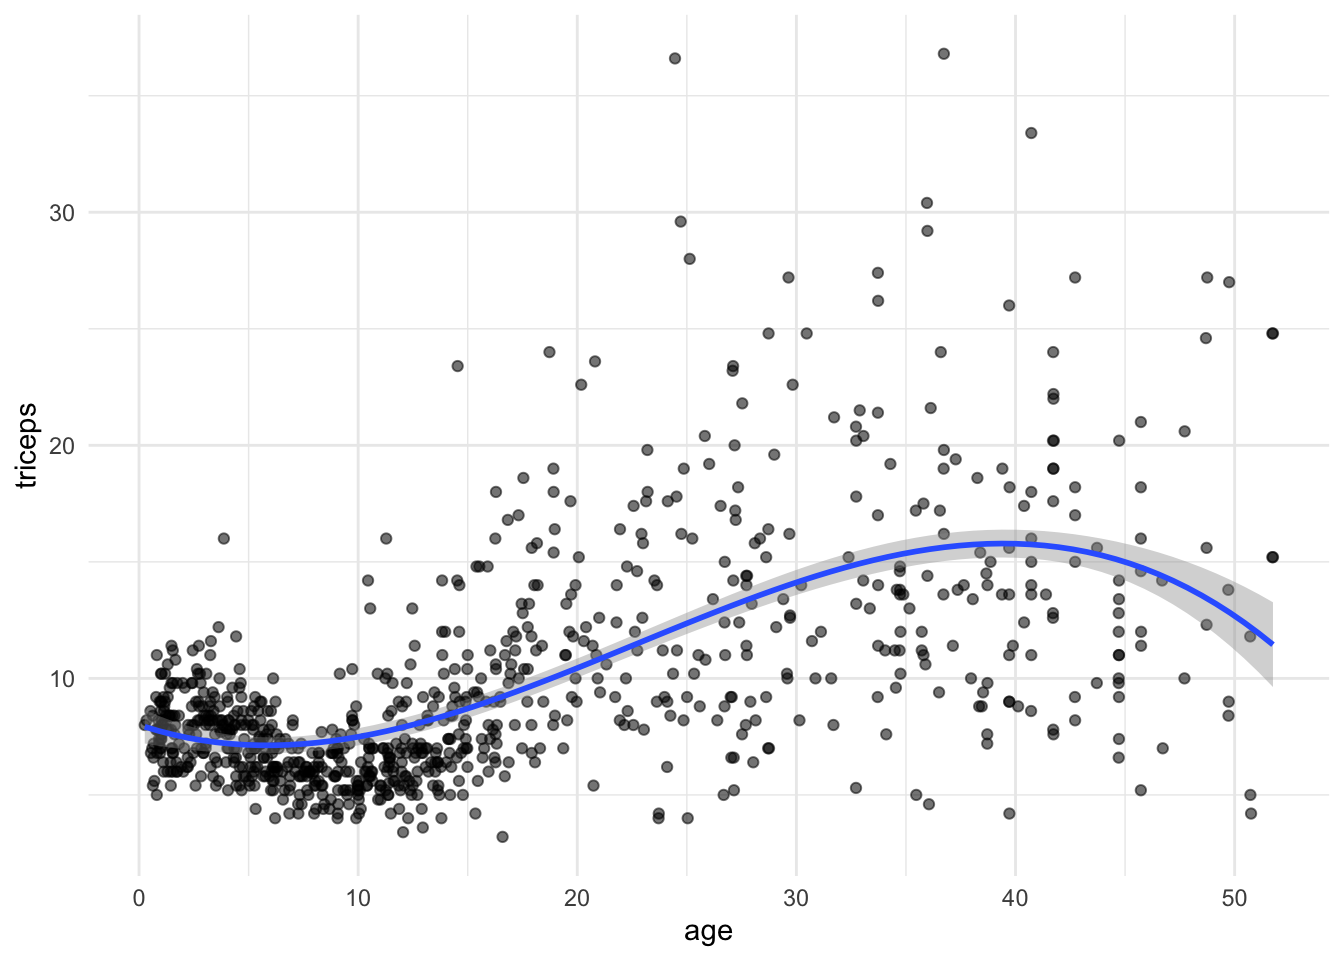
\includegraphics[keepaspectratio]{_main_files/figure-latex/fitcubic-1.pdf}}

\textbf{TRY IT YOURSELF:}

\begin{enumerate}
\def\labelenumi{\arabic{enumi})}
\tightlist
\item
  Add a linear fit to the plot above
\end{enumerate}

See the solution code

\begin{Shaded}
\begin{Highlighting}[]
\NormalTok{ tri.age.plot }\SpecialCharTok{+} 
   \FunctionTok{stat\_smooth}\NormalTok{(}\AttributeTok{method =} \StringTok{"lm"}\NormalTok{, }
               \AttributeTok{formula =}\NormalTok{ y}\SpecialCharTok{\textasciitilde{}}\FunctionTok{poly}\NormalTok{(x,}\DecValTok{3}\NormalTok{,}\AttributeTok{raw=}\NormalTok{T), }\AttributeTok{size =} \DecValTok{1}\NormalTok{) }\SpecialCharTok{+}
     \FunctionTok{stat\_smooth}\NormalTok{(}\AttributeTok{method =} \StringTok{"lm"}\NormalTok{, }
               \AttributeTok{formula =}\NormalTok{ y}\SpecialCharTok{\textasciitilde{}}\FunctionTok{poly}\NormalTok{(x,}\DecValTok{1}\NormalTok{,}\AttributeTok{raw=}\NormalTok{T), }\AttributeTok{lty =} \DecValTok{2}\NormalTok{, }\AttributeTok{col =} \StringTok{"red"}\NormalTok{ , }\AttributeTok{size =} \DecValTok{1}\NormalTok{)}
\end{Highlighting}
\end{Shaded}

\pandocbounded{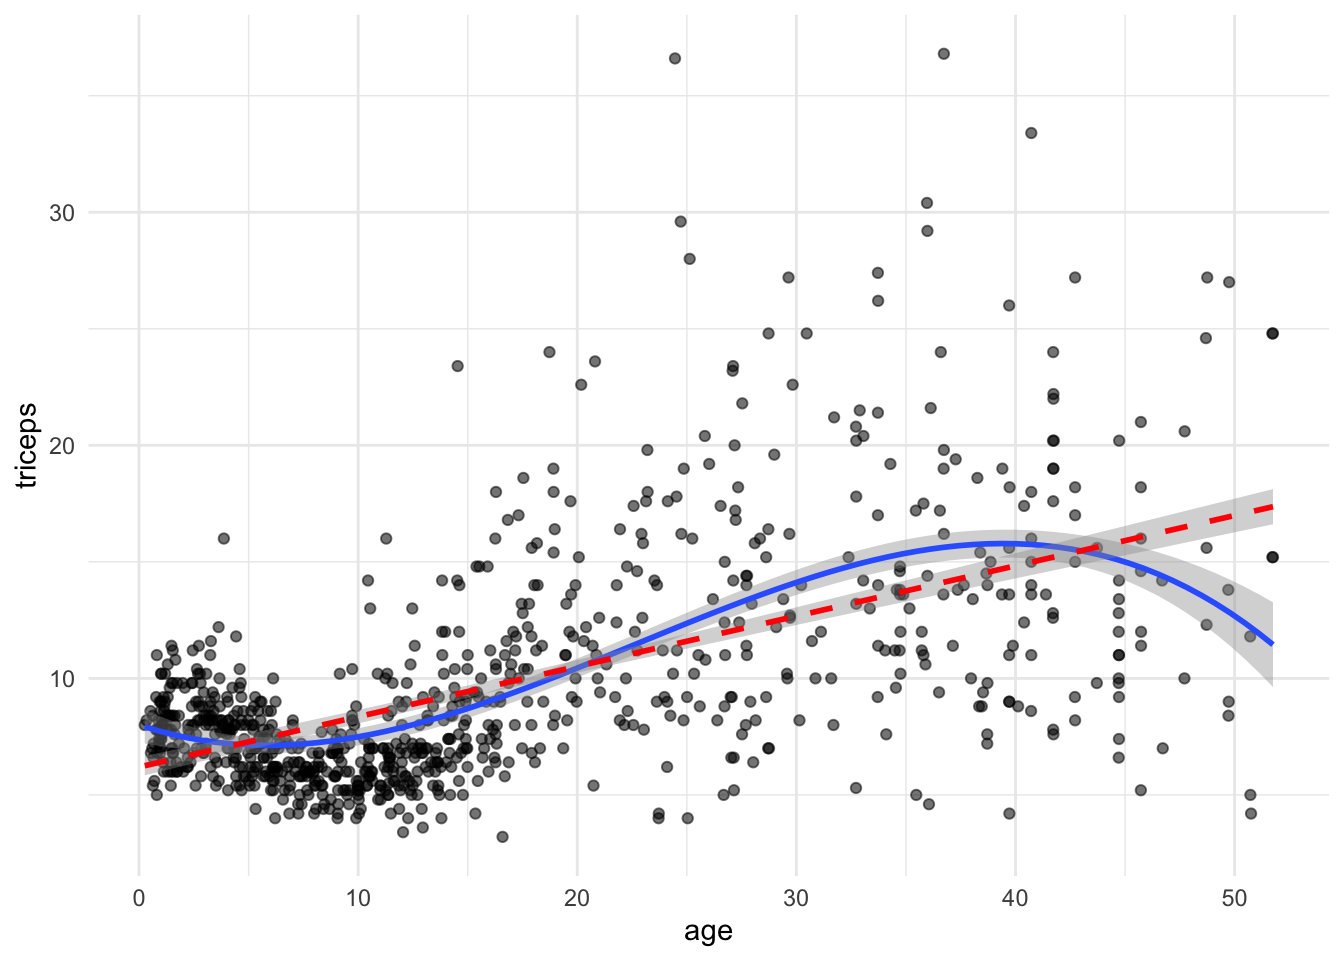
\includegraphics[keepaspectratio]{_main_files/figure-latex/lincub-1.pdf}}

\subsection*{Task 2 - Mean Squared Error for the quadratic model}\label{task-2---mean-squared-error-for-the-quadratic-model}
\addcontentsline{toc}{subsection}{Task 2 - Mean Squared Error for the quadratic model}

We will use the same dataset and the same variables as in TASK 1 but now we
want to compute the cross-validated MSE for the quadratic model

There are multiple ways of doing this. We will take advantage of the
easy implementation of cross-validation in the \texttt{caret} package. We will do
10-fold cross-validations and repeat it 10 times:

\begin{Shaded}
\begin{Highlighting}[]
\FunctionTok{library}\NormalTok{(caret)}
\end{Highlighting}
\end{Shaded}

\begin{verbatim}
## Loading required package: lattice
\end{verbatim}

\begin{verbatim}
## Registered S3 method overwritten by 'future':
##   method               from      
##   all.equal.connection parallelly
\end{verbatim}

\begin{Shaded}
\begin{Highlighting}[]
\FunctionTok{set.seed}\NormalTok{(}\DecValTok{1234}\NormalTok{)}

\CommentTok{\#repeated CV for the MSE}
\NormalTok{trC.lm }\OtherTok{\textless{}{-}} \FunctionTok{trainControl}\NormalTok{(}\AttributeTok{method =} \StringTok{"repeatedcv"}\NormalTok{, }
                       \AttributeTok{number =} \DecValTok{10}\NormalTok{,         }\CommentTok{\#10{-}fold cross{-}validation}
                       \AttributeTok{repeats =} \DecValTok{10}\NormalTok{)        }\CommentTok{\#10 times}
  
\CommentTok{\#function to fit a polynomial model of degree x}
\NormalTok{pol.model }\OtherTok{\textless{}{-}} \FunctionTok{train}\NormalTok{(triceps }\SpecialCharTok{\textasciitilde{}} \FunctionTok{poly}\NormalTok{(age,}\DecValTok{2}\NormalTok{),}
                       \AttributeTok{data =}\NormalTok{ triceps, }
                       \AttributeTok{method =} \StringTok{"lm"}\NormalTok{,}
                       \AttributeTok{trControl =}\NormalTok{ trC.lm)}
    
 \CommentTok{\#this is the root mean squared error}
\NormalTok{  pol.model}\SpecialCharTok{$}\NormalTok{results[}\DecValTok{2}\NormalTok{]                      }
\end{Highlighting}
\end{Shaded}

\begin{verbatim}
##       RMSE
## 1 3.988524
\end{verbatim}

\textbf{TRY IT YOURSELF:}

\begin{enumerate}
\def\labelenumi{\arabic{enumi})}
\tightlist
\item
  Calculate the MSE (or the root mean squared error) for the model using
  a degree 4 polynomial, through cross-validation
\end{enumerate}

See the solution code

\begin{Shaded}
\begin{Highlighting}[]
\FunctionTok{set.seed}\NormalTok{(}\DecValTok{1001}\NormalTok{)}

\CommentTok{\#repeated CV for the MSE}
\NormalTok{trC.lm }\OtherTok{\textless{}{-}} \FunctionTok{trainControl}\NormalTok{(}\AttributeTok{method =} \StringTok{"repeatedcv"}\NormalTok{, }
                       \AttributeTok{number =} \DecValTok{10}\NormalTok{,         }\CommentTok{\#10{-}fold cross{-}validation}
                       \AttributeTok{repeats =} \DecValTok{10}\NormalTok{)        }\CommentTok{\#10 times}
  
\CommentTok{\#function to fit a polynomial model of degree x}
\NormalTok{pol.model }\OtherTok{\textless{}{-}} \FunctionTok{train}\NormalTok{(triceps }\SpecialCharTok{\textasciitilde{}} \FunctionTok{poly}\NormalTok{(age,}\DecValTok{4}\NormalTok{),}
                       \AttributeTok{data =}\NormalTok{ triceps, }
                       \AttributeTok{method =} \StringTok{"lm"}\NormalTok{,}
                       \AttributeTok{trControl =}\NormalTok{ trC.lm)}
    
 \CommentTok{\#this is the root mean squared error}
\NormalTok{  pol.model}\SpecialCharTok{$}\NormalTok{results[}\DecValTok{2}\NormalTok{]                      }
\end{Highlighting}
\end{Shaded}

\begin{verbatim}
##       RMSE
## 1 3.782918
\end{verbatim}

\begin{enumerate}
\def\labelenumi{\arabic{enumi})}
\setcounter{enumi}{1}
\tightlist
\item
  Calculate the MSE (or the root mean squared error) for the models using
  polynomials from degree 1 (linear) up to 10
\end{enumerate}

See the solution code

\begin{Shaded}
\begin{Highlighting}[]
\FunctionTok{set.seed}\NormalTok{(}\DecValTok{1001}\NormalTok{)}
   \CommentTok{\#repeated CV for the MSE}
\NormalTok{  trC.lm }\OtherTok{\textless{}{-}} \FunctionTok{trainControl}\NormalTok{(}\AttributeTok{method =} \StringTok{"repeatedcv"}\NormalTok{, }
                         \AttributeTok{number =} \DecValTok{10}\NormalTok{, }
                         \AttributeTok{repeats =} \DecValTok{10}\NormalTok{)}

  \CommentTok{\#function to fit a polynomial model of degree x}
\NormalTok{  my.pol.f }\OtherTok{\textless{}{-}} \ControlFlowTok{function}\NormalTok{(x) \{}
\NormalTok{    xx}\OtherTok{\textless{}{-}}\FunctionTok{poly}\NormalTok{(triceps}\SpecialCharTok{$}\NormalTok{age, x, }\AttributeTok{raw=}\NormalTok{T)                   }\CommentTok{\#design matrix with age,}
                                                      \CommentTok{\#age\^{}2, ..., age\^{}10}
\NormalTok{    new.data  }\OtherTok{\textless{}{-}} \FunctionTok{cbind}\NormalTok{(}\AttributeTok{triceps=}\NormalTok{triceps}\SpecialCharTok{$}\NormalTok{triceps, xx)   }\CommentTok{\#dataset with the added}
                                                      \CommentTok{\#poly terms}
\NormalTok{    pol.model }\OtherTok{\textless{}{-}} \FunctionTok{train}\NormalTok{(triceps }\SpecialCharTok{\textasciitilde{}}\NormalTok{ .,                   }\CommentTok{\#the . uses all the }
                          \AttributeTok{data =}\NormalTok{ new.data,            }\CommentTok{\#predictors}
                          \AttributeTok{method =} \StringTok{"lm"}\NormalTok{,}
                          \AttributeTok{trControl =}\NormalTok{ trC.lm)}
    
\NormalTok{    RMSE.cv }\OtherTok{=}\NormalTok{ pol.model}\SpecialCharTok{$}\NormalTok{results[}\DecValTok{2}\NormalTok{]}
\NormalTok{  \}}
  
    \CommentTok{\#RMSE}
  \FunctionTok{t}\NormalTok{(}\FunctionTok{sapply}\NormalTok{(}\DecValTok{1}\SpecialCharTok{:}\DecValTok{10}\NormalTok{, my.pol.f))                        }\CommentTok{\#applies the function}
                                                   \CommentTok{\#to poly degrees 1 to 10}
\end{Highlighting}
\end{Shaded}

\section{Exercises}\label{PR4}

Solve the following exercise:

\begin{enumerate}
\def\labelenumi{\arabic{enumi})}
\tightlist
\item
  The dataset \href{https://www.dropbox.com/s/cwkw3p91zyizcqz/SA_heart.csv?dl=1}{SA\_heart.csv}
  contains on coronary heart disease status (variable \emph{chd}) and several risk
  factors including the cumulative tobacco comsumption \emph{tobacco}.
\end{enumerate}

\begin{enumerate}
\def\labelenumi{\alph{enumi})}
\item
  Fit a logistic model for \emph{chd} using the predictor \emph{tobacco}
  (as a linear effect) and compute its AIC
\item
  Plot the fitted curve in a)
\item
  Fit a logistic model for \emph{chd} allowing a cubic effect of the
  predictor \emph{tobacco} and compute its AIC.
\item
  Plot the fitted curve in c)
\item
  Compute the cross-validated ROC of the models a) and c) (use the \texttt{caret}
  package)
\end{enumerate}

See the solution code for e)

\begin{Shaded}
\begin{Highlighting}[]
    \FunctionTok{library}\NormalTok{(caret)}
    \FunctionTok{set.seed}\NormalTok{(}\DecValTok{2001}\NormalTok{)}
\NormalTok{    SA\_heart }\OtherTok{\textless{}{-}} \FunctionTok{read.csv}\NormalTok{(}\StringTok{"https://www.dropbox.com/s/cwkw3p91zyizcqz/SA\_heart.csv?dl=1"}\NormalTok{)}
    
    \CommentTok{\# caret will give an error for factors coded as 0 and 1}
    \CommentTok{\# because it uses the factors names to create}
    \CommentTok{\# names of internal variables. This way it is better}
    \CommentTok{\#to use an outcome variable with strings as the factor names}
\NormalTok{    SA\_heart}\SpecialCharTok{$}\NormalTok{chd.f }\OtherTok{\textless{}{-}} \FunctionTok{ifelse}\NormalTok{(SA\_heart}\SpecialCharTok{$}\NormalTok{chd }\SpecialCharTok{==}\DecValTok{1}\NormalTok{, }
                             \StringTok{"chd"}\NormalTok{, }
                             \StringTok{"nochd"}\NormalTok{)     }
    
    \CommentTok{\#sets the control for 10{-}fold cross{-}validation, 10 times}
    \CommentTok{\# the classProbs = TRUE and summaryFunction = twoClassSummary}
    \CommentTok{\# store the information to compute the area under the ROC}
\NormalTok{    trC.lm }\OtherTok{\textless{}{-}} \FunctionTok{trainControl}\NormalTok{(}\AttributeTok{method =} \StringTok{"repeatedcv"}\NormalTok{, }
                           \AttributeTok{number =} \DecValTok{10}\NormalTok{, }
                           \AttributeTok{repeats =} \DecValTok{10}\NormalTok{,}
                           \AttributeTok{classProbs =} \ConstantTok{TRUE}\NormalTok{,                 }\CommentTok{\#necessary for }
                           \AttributeTok{summaryFunction =}\NormalTok{ twoClassSummary) }\CommentTok{\#the AUC ROC}

     \CommentTok{\#linear effect}
\NormalTok{     roc.l }\OtherTok{\textless{}{-}} \FunctionTok{train}\NormalTok{(}\AttributeTok{form =}\NormalTok{ chd.f  }\SpecialCharTok{\textasciitilde{}}\NormalTok{ tobacco,}
                    \AttributeTok{data =}\NormalTok{ SA\_heart,}
                    \AttributeTok{method =} \StringTok{"glm"}\NormalTok{,}
                    \AttributeTok{family =} \StringTok{"binomial"}\NormalTok{,}
                    \AttributeTok{trControl =}\NormalTok{ trC.lm,}
                    \AttributeTok{metric =} \StringTok{"ROC"}\NormalTok{) }
     \CommentTok{\#cubic effect}
\NormalTok{     roc.c }\OtherTok{\textless{}{-}} \FunctionTok{train}\NormalTok{(}\AttributeTok{form =}\NormalTok{ chd.f  }\SpecialCharTok{\textasciitilde{}} \FunctionTok{poly}\NormalTok{(tobacco,}\DecValTok{3}\NormalTok{),}
                    \AttributeTok{data =}\NormalTok{ SA\_heart,}
                    \AttributeTok{method =} \StringTok{"glm"}\NormalTok{,}
                    \AttributeTok{family =} \StringTok{"binomial"}\NormalTok{,}
                    \AttributeTok{trControl =}\NormalTok{ trC.lm,}
                    \AttributeTok{metric =} \StringTok{"ROC"}\NormalTok{) }
  
\NormalTok{     roc.l }
\NormalTok{     roc.c}
\end{Highlighting}
\end{Shaded}

\begin{enumerate}
\def\labelenumi{\alph{enumi})}
\setcounter{enumi}{5}
\tightlist
\item
  Which model would you prefer?
\end{enumerate}

\chapter{Piecewise Regression and Splines}\label{piecewise-regression-and-splines}

\section{Introduction}\label{PWR1}

An alternative to fitting all data points with a single polynomial curve, is to
fit segments to different parts of the data, with breakpoints (knots) at
pre-determined places.

\pandocbounded{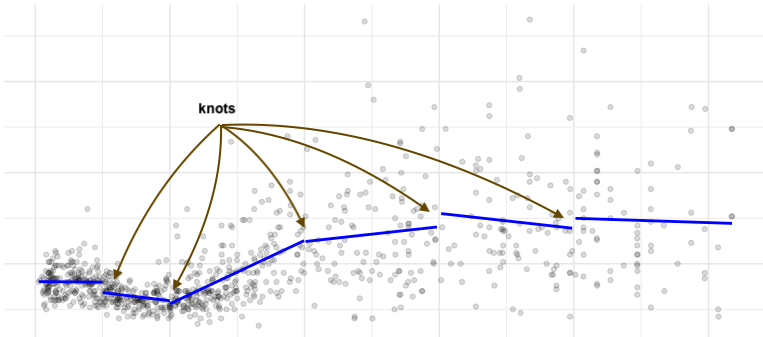
\includegraphics[keepaspectratio]{piece1.png}}

We can further require continuity, meaning that the segments have to
be connected

\pandocbounded{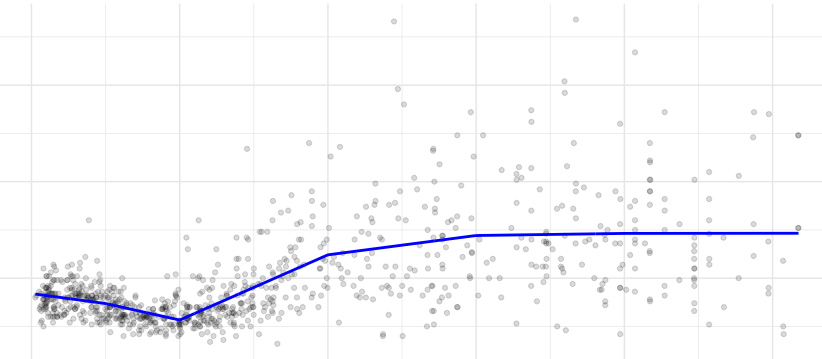
\includegraphics[keepaspectratio]{piece2.png}}
Again, the knots need to be specified and the regression equation becomes:

\[
y = \beta_0 + \beta_1 x +  \beta_2 (x-k_1)_{+}  + \beta_3 (x-k_2)_{+} + ... + \beta_6 (x-k_p)_{+} + \varepsilon\\
\]

where
\[(x-k)_{+} =  \begin{cases}
                  0, & \text{ if  } x < k \\
                  x-k, & \text{ if  } x \geq k\\
                 \end{cases} 
\]

The approach above may be extended to use polynomial segments. For example,
using cubic segments, the model would become

\[
y = \beta_0 + \beta_1 x +  \beta_2 x^2 + \beta_3 x^3 + \beta_4 (x-k_1)_{+} + \beta_5 (x-k_1)^2_{+} + \beta_6 (x-k_1)^3_{+}   + ... +  \varepsilon
\]

The above model will be a smooth curve within the intervals bounded by the
knots, but the ``connection'' between the segments will not be smooth. To force
smoothness over the entire fitted curve we can restrict the the model above to
only include the cubic components:

\[
y = \beta_0 + \beta_1 x +  \beta_2 x^2 + \beta_3 x^3 + \beta_4 (x-k_1)^3_{+} + \beta_5 (x-k_2)^3_{+} + \beta_6 (x-k_3)^3_{+}   + ... +  \varepsilon
\]

This will guarantee that the fitted curve is differentiable, with no sharp
changes in the direction. This is called a cubic spline.

An improvement of the fitting of splines in the boundary of the data is
achieved by using linear fitting before the first knot and after the last one.

\section{Readings}\label{PWR2}

Read the following chapters of \emph{An introduction to statistical learning}:

\begin{itemize}
\tightlist
\item
  7.2 Step Functions
\item
  7.3 Basis Functions
\item
  7.4 Regression Splines
\end{itemize}

\section{Practice session}\label{PWR3}

\subsection*{Task 1 - Fit a piecewise linear regression}\label{task-1---fit-a-piecewise-linear-regression}
\addcontentsline{toc}{subsection}{Task 1 - Fit a piecewise linear regression}

We will continue the example using the dataset \textbf{triceps} available in the \texttt{MultiKink} package. The data contains the measurement of the triceps skin fold of 892 females (variable \emph{triceps}) and we want to model its association with \textbf{age}, using piecewise linear regression with knots at 5,10,20,30 and 40.

First, we will load the data

\begin{Shaded}
\begin{Highlighting}[]
\CommentTok{\#libraries that we will need}
\CommentTok{\#install.packages("MultiKink")  }
\FunctionTok{library}\NormalTok{(MultiKink) }\CommentTok{\#for the data}
\FunctionTok{library}\NormalTok{(ggplot2)   }\CommentTok{\#for the plots}
\FunctionTok{set.seed}\NormalTok{(}\DecValTok{1974}\NormalTok{)     }\CommentTok{\#fix the random generator seed }

\FunctionTok{data}\NormalTok{(}\StringTok{"triceps"}\NormalTok{)   }\CommentTok{\#load the dataset triceps}
                  \CommentTok{\#notice that the variable of interest}
                  \CommentTok{\#it is also called tricets. Don\textquotesingle{}t get }
                  \CommentTok{\#confused!}
\end{Highlighting}
\end{Shaded}

And plot the scatter for \textbf{triceps} and \textbf{age}

\begin{Shaded}
\begin{Highlighting}[]
 \CommentTok{\#simple scatter}
  \CommentTok{\#we can store the scatter in an object }
  \CommentTok{\#to use it later}
\NormalTok{ tri.age.plot }\OtherTok{\textless{}{-}} \FunctionTok{ggplot}\NormalTok{(triceps, }\FunctionTok{aes}\NormalTok{(}\AttributeTok{x=}\NormalTok{age, }\AttributeTok{y=}\NormalTok{triceps)) }\SpecialCharTok{+}
                 \FunctionTok{geom\_point}\NormalTok{(}\AttributeTok{alpha=}\FloatTok{0.55}\NormalTok{, }\AttributeTok{color=}\StringTok{"black"}\NormalTok{) }\SpecialCharTok{+} 
                 \FunctionTok{theme\_minimal}\NormalTok{() }
\NormalTok{ tri.age.plot}
\end{Highlighting}
\end{Shaded}

\pandocbounded{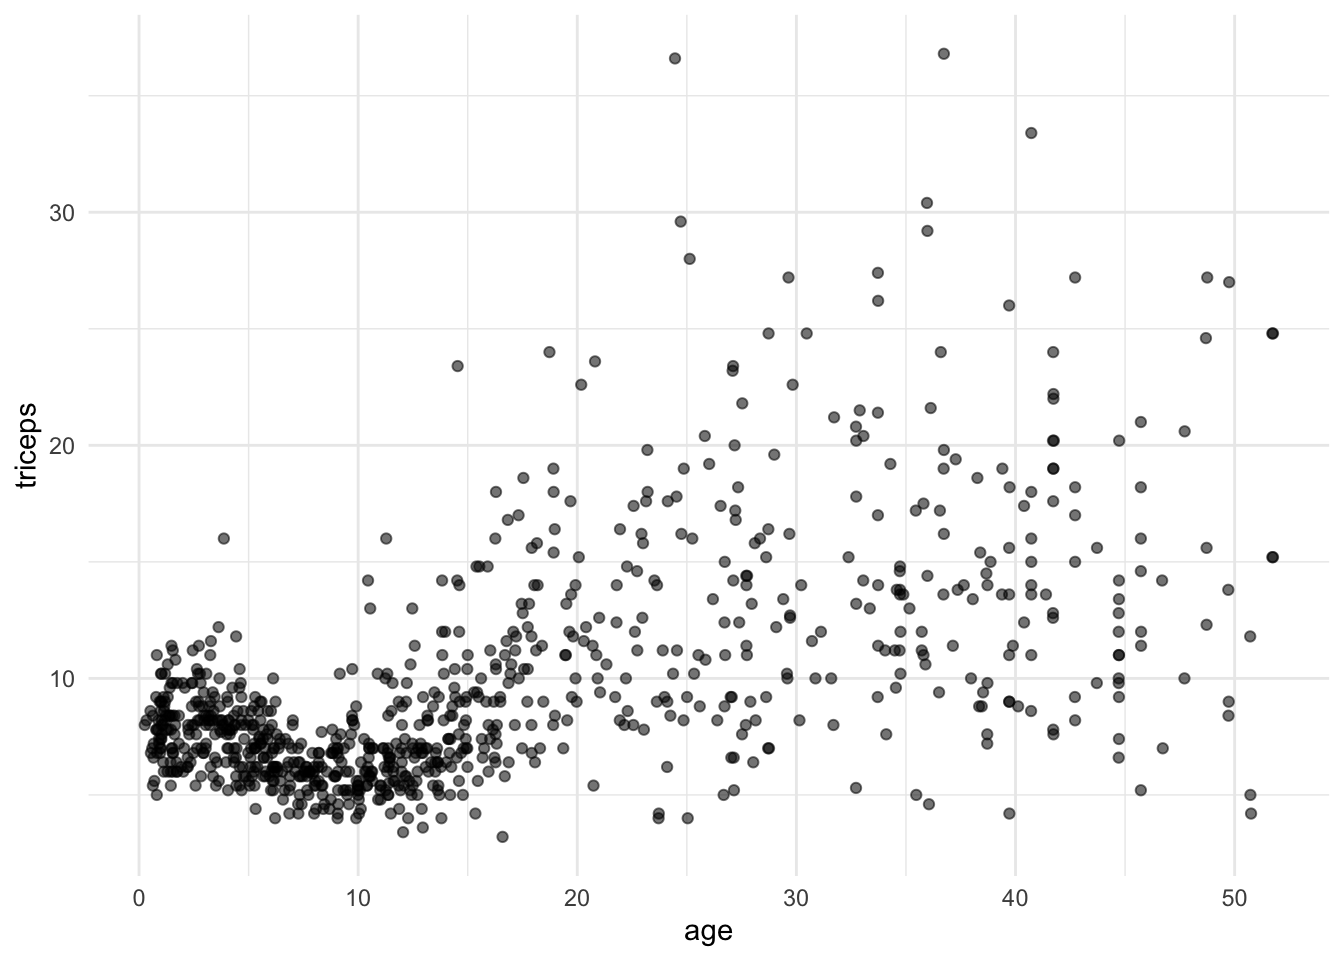
\includegraphics[keepaspectratio]{_main_files/figure-latex/plotagetric1-1.pdf}}

We will fit linear models within the intervals defined by the knots. The \texttt{predict()} will give us the fitted lines.

\begin{Shaded}
\begin{Highlighting}[]
\DocumentationTok{\#\#\#Piecewise regression}

\NormalTok{pred1 }\OtherTok{\textless{}{-}} \FunctionTok{predict}\NormalTok{(}\FunctionTok{lm}\NormalTok{(triceps}\SpecialCharTok{\textasciitilde{}}\NormalTok{age, }
                    \AttributeTok{data =}\NormalTok{ triceps[triceps}\SpecialCharTok{$}\NormalTok{age}\SpecialCharTok{\textless{}}\DecValTok{5}\NormalTok{,]))}
\NormalTok{pred2 }\OtherTok{\textless{}{-}} \FunctionTok{predict}\NormalTok{(}\FunctionTok{lm}\NormalTok{(triceps}\SpecialCharTok{\textasciitilde{}}\NormalTok{age, }
                    \AttributeTok{data =}\NormalTok{ triceps[triceps}\SpecialCharTok{$}\NormalTok{age }\SpecialCharTok{\textgreater{}=}\DecValTok{5} \SpecialCharTok{\&}\NormalTok{ triceps}\SpecialCharTok{$}\NormalTok{age}\SpecialCharTok{\textless{}}\DecValTok{10}\NormalTok{,]))}
\NormalTok{pred3 }\OtherTok{\textless{}{-}} \FunctionTok{predict}\NormalTok{(}\FunctionTok{lm}\NormalTok{(triceps}\SpecialCharTok{\textasciitilde{}}\NormalTok{age, }
                    \AttributeTok{data =}\NormalTok{ triceps[triceps}\SpecialCharTok{$}\NormalTok{age}\SpecialCharTok{\textgreater{}=}\DecValTok{10} \SpecialCharTok{\&}\NormalTok{ triceps}\SpecialCharTok{$}\NormalTok{age}\SpecialCharTok{\textless{}}\DecValTok{20}\NormalTok{,]))}
\NormalTok{pred4 }\OtherTok{\textless{}{-}} \FunctionTok{predict}\NormalTok{(}\FunctionTok{lm}\NormalTok{(triceps}\SpecialCharTok{\textasciitilde{}}\NormalTok{age, }
                    \AttributeTok{data =}\NormalTok{ triceps[triceps}\SpecialCharTok{$}\NormalTok{age}\SpecialCharTok{\textgreater{}=}\DecValTok{20} \SpecialCharTok{\&}\NormalTok{ triceps}\SpecialCharTok{$}\NormalTok{age}\SpecialCharTok{\textless{}}\DecValTok{30}\NormalTok{,]))}
\NormalTok{pred5 }\OtherTok{\textless{}{-}} \FunctionTok{predict}\NormalTok{(}\FunctionTok{lm}\NormalTok{(triceps}\SpecialCharTok{\textasciitilde{}}\NormalTok{age, }
                    \AttributeTok{data =}\NormalTok{ triceps[triceps}\SpecialCharTok{$}\NormalTok{age}\SpecialCharTok{\textgreater{}=}\DecValTok{30} \SpecialCharTok{\&}\NormalTok{ triceps}\SpecialCharTok{$}\NormalTok{age}\SpecialCharTok{\textless{}}\DecValTok{40}\NormalTok{,]))}
\NormalTok{pred6 }\OtherTok{\textless{}{-}} \FunctionTok{predict}\NormalTok{(}\FunctionTok{lm}\NormalTok{(triceps}\SpecialCharTok{\textasciitilde{}}\NormalTok{age, }
                    \AttributeTok{data =}\NormalTok{ triceps[triceps}\SpecialCharTok{$}\NormalTok{age}\SpecialCharTok{\textgreater{}=}\DecValTok{40}\NormalTok{,]))}
\end{Highlighting}
\end{Shaded}

And we can now add the segments to the scatter plot

\begin{Shaded}
\begin{Highlighting}[]
\NormalTok{tri.age.plot }\SpecialCharTok{+} 
  \FunctionTok{geom\_line}\NormalTok{(}\AttributeTok{data=}\NormalTok{triceps[triceps}\SpecialCharTok{$}\NormalTok{age}\SpecialCharTok{\textless{}}\DecValTok{5}\NormalTok{,], }
            \FunctionTok{aes}\NormalTok{(}\AttributeTok{y =}\NormalTok{ pred1, }\AttributeTok{x=}\NormalTok{age), }\AttributeTok{size =} \DecValTok{1}\NormalTok{, }\AttributeTok{col=}\StringTok{"blue"}\NormalTok{) }\SpecialCharTok{+}
  \FunctionTok{geom\_line}\NormalTok{(}\AttributeTok{data=}\NormalTok{triceps[triceps}\SpecialCharTok{$}\NormalTok{age }\SpecialCharTok{\textgreater{}=}\DecValTok{5} \SpecialCharTok{\&}\NormalTok{ triceps}\SpecialCharTok{$}\NormalTok{age}\SpecialCharTok{\textless{}}\DecValTok{10}\NormalTok{,], }
            \FunctionTok{aes}\NormalTok{(}\AttributeTok{y =}\NormalTok{ pred2, }\AttributeTok{x=}\NormalTok{age), }\AttributeTok{size =} \DecValTok{1}\NormalTok{, }\AttributeTok{col=}\StringTok{"blue"}\NormalTok{) }\SpecialCharTok{+}
  \FunctionTok{geom\_line}\NormalTok{(}\AttributeTok{data=}\NormalTok{triceps[triceps}\SpecialCharTok{$}\NormalTok{age}\SpecialCharTok{\textgreater{}=}\DecValTok{10} \SpecialCharTok{\&}\NormalTok{ triceps}\SpecialCharTok{$}\NormalTok{age}\SpecialCharTok{\textless{}}\DecValTok{20}\NormalTok{,], }
            \FunctionTok{aes}\NormalTok{(}\AttributeTok{y =}\NormalTok{ pred3, }\AttributeTok{x=}\NormalTok{age), }\AttributeTok{size =} \DecValTok{1}\NormalTok{, }\AttributeTok{col=}\StringTok{"blue"}\NormalTok{) }\SpecialCharTok{+}
  \FunctionTok{geom\_line}\NormalTok{(}\AttributeTok{data=}\NormalTok{triceps[triceps}\SpecialCharTok{$}\NormalTok{age}\SpecialCharTok{\textgreater{}=}\DecValTok{20} \SpecialCharTok{\&}\NormalTok{ triceps}\SpecialCharTok{$}\NormalTok{age}\SpecialCharTok{\textless{}}\DecValTok{30}\NormalTok{,], }
            \FunctionTok{aes}\NormalTok{(}\AttributeTok{y =}\NormalTok{ pred4, }\AttributeTok{x=}\NormalTok{age), }\AttributeTok{size =} \DecValTok{1}\NormalTok{, }\AttributeTok{col=}\StringTok{"blue"}\NormalTok{) }\SpecialCharTok{+}
  \FunctionTok{geom\_line}\NormalTok{(}\AttributeTok{data=}\NormalTok{triceps[triceps}\SpecialCharTok{$}\NormalTok{age}\SpecialCharTok{\textgreater{}=}\DecValTok{30} \SpecialCharTok{\&}\NormalTok{ triceps}\SpecialCharTok{$}\NormalTok{age}\SpecialCharTok{\textless{}}\DecValTok{40}\NormalTok{,], }
            \FunctionTok{aes}\NormalTok{(}\AttributeTok{y =}\NormalTok{ pred5, }\AttributeTok{x=}\NormalTok{age), }\AttributeTok{size =} \DecValTok{1}\NormalTok{, }\AttributeTok{col=}\StringTok{"blue"}\NormalTok{) }\SpecialCharTok{+}
  \FunctionTok{geom\_line}\NormalTok{(}\AttributeTok{data=}\NormalTok{triceps[triceps}\SpecialCharTok{$}\NormalTok{age}\SpecialCharTok{\textgreater{}=}\DecValTok{40}\NormalTok{,], }
            \FunctionTok{aes}\NormalTok{(}\AttributeTok{y =}\NormalTok{ pred6, }\AttributeTok{x=}\NormalTok{age), }\AttributeTok{size =} \DecValTok{1}\NormalTok{, }\AttributeTok{col=}\StringTok{"blue"}\NormalTok{) }
\end{Highlighting}
\end{Shaded}

\pandocbounded{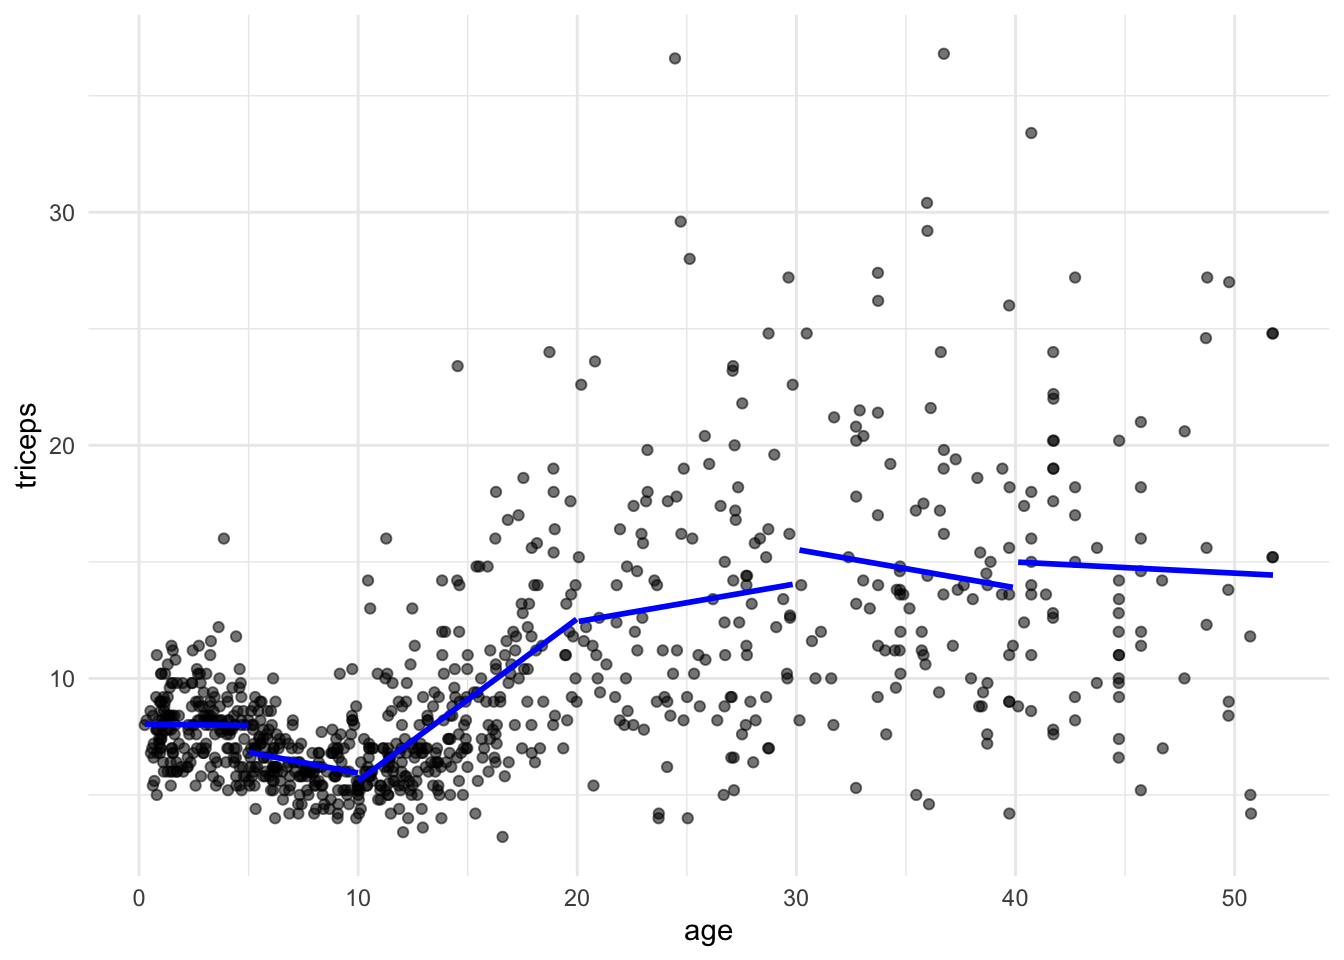
\includegraphics[keepaspectratio]{_main_files/figure-latex/unnamed-chunk-10-1.pdf}}

We can restrict the segments to be connected, i.e., to fit a continuous line. The model is

\[
y = \beta_0 + \beta_1 x +  \beta_2 (x-k_1)_{+}  + \beta_3 (x-k_2)_{+} + ... + \beta_6 (x-k_p)_{+} + \varepsilon\\
\]

where
\[(x-k)_{+} =  \begin{cases}
                  0, & \text{ if  } x < k \\
                  x-k, & \text{ if  } x \geq k\\
                 \end{cases} 
\]

So, we need to add the terms \((x-k)\) when \(x \geq k\). We will do this by adding \(I((age-k)*(age >= k))\) terms to the linear model. Note that \((age >= k)\) is a logical statement that will be 0 (\(FALSE\)) of 1 (\(TRUE\)) and I() evaluates that all expression.

\begin{Shaded}
\begin{Highlighting}[]
\NormalTok{pred7 }\OtherTok{\textless{}{-}} \FunctionTok{predict}\NormalTok{(}\FunctionTok{lm}\NormalTok{(triceps}\SpecialCharTok{\textasciitilde{}}\NormalTok{ age }\SpecialCharTok{+} \FunctionTok{I}\NormalTok{((age}\DecValTok{{-}5}\NormalTok{)}\SpecialCharTok{*}\NormalTok{(age}\SpecialCharTok{\textgreater{}=}\DecValTok{5}\NormalTok{)) }\SpecialCharTok{+}
                                   \FunctionTok{I}\NormalTok{((age}\DecValTok{{-}10}\NormalTok{)}\SpecialCharTok{*}\NormalTok{(age }\SpecialCharTok{\textgreater{}=} \DecValTok{10}\NormalTok{)) }\SpecialCharTok{+}
                                   \FunctionTok{I}\NormalTok{((age}\DecValTok{{-}20}\NormalTok{)}\SpecialCharTok{*}\NormalTok{(age }\SpecialCharTok{\textgreater{}=} \DecValTok{20}\NormalTok{)) }\SpecialCharTok{+}
                                   \FunctionTok{I}\NormalTok{((age}\DecValTok{{-}30}\NormalTok{)}\SpecialCharTok{*}\NormalTok{(age }\SpecialCharTok{\textgreater{}=} \DecValTok{30}\NormalTok{)) }\SpecialCharTok{+}
                                  \FunctionTok{I}\NormalTok{((age}\DecValTok{{-}40}\NormalTok{)}\SpecialCharTok{*}\NormalTok{(age }\SpecialCharTok{\textgreater{}=} \DecValTok{40}\NormalTok{)),}
                    \AttributeTok{data =}\NormalTok{ triceps))}

\NormalTok{tri.age.plot }\SpecialCharTok{+}
  \FunctionTok{geom\_line}\NormalTok{(}\AttributeTok{data=}\NormalTok{triceps, }
            \FunctionTok{aes}\NormalTok{(}\AttributeTok{y =}\NormalTok{ pred7, }\AttributeTok{x=}\NormalTok{age), }\AttributeTok{size =} \DecValTok{1}\NormalTok{, }\AttributeTok{col=}\StringTok{"blue"}\NormalTok{) }
\end{Highlighting}
\end{Shaded}

\pandocbounded{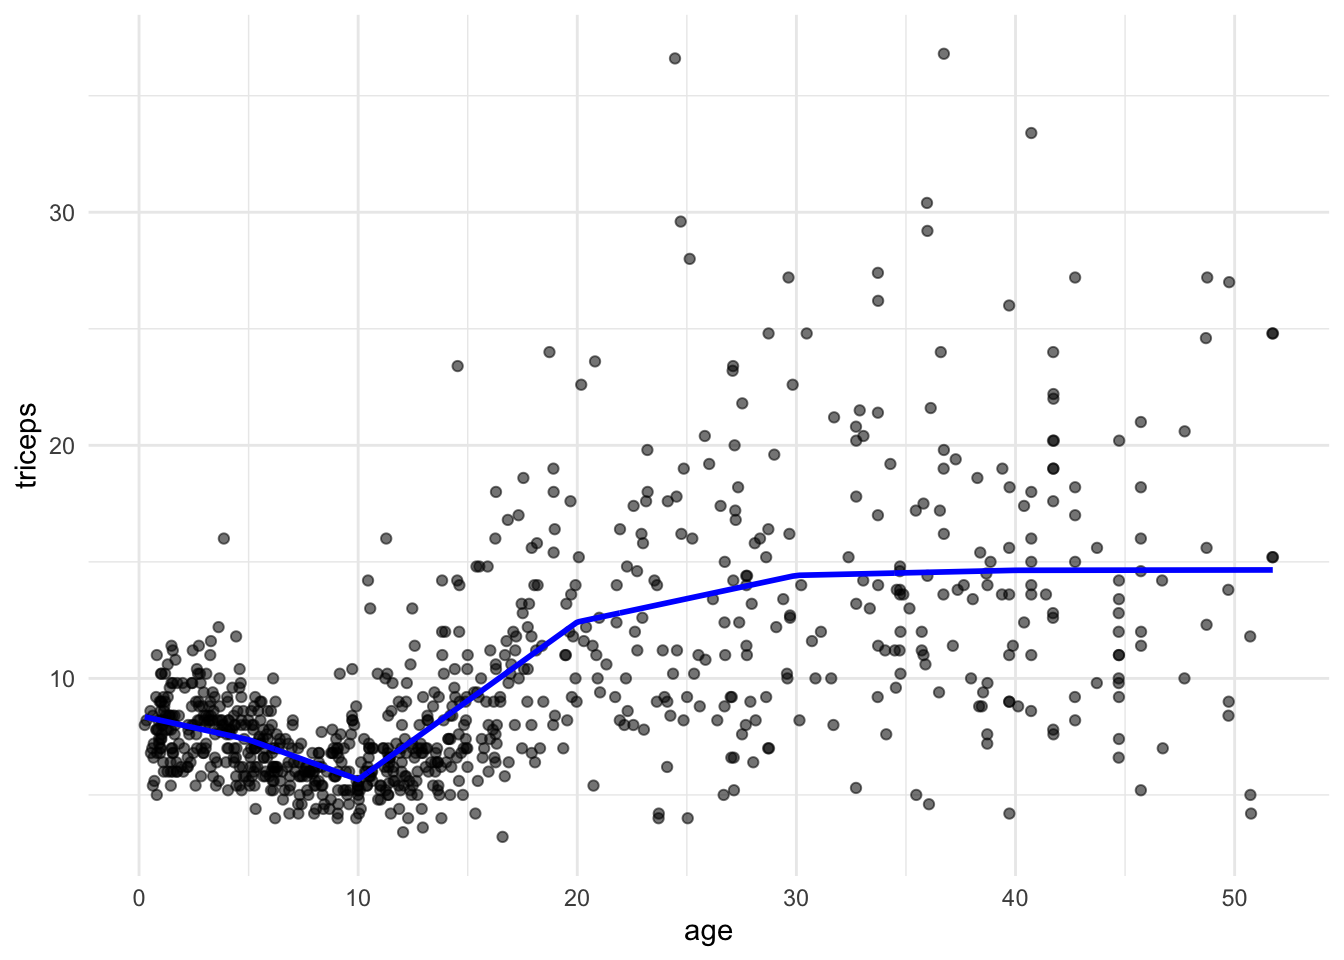
\includegraphics[keepaspectratio]{_main_files/figure-latex/jointpiece-1.pdf}}

\textbf{TRY IT YOURSELF:}

\begin{enumerate}
\def\labelenumi{\arabic{enumi})}
\tightlist
\item
  Using the same knots as above, fit a quadratic piecewise regression
\end{enumerate}

See the solution code

\begin{Shaded}
\begin{Highlighting}[]
\NormalTok{ pred.quad }\OtherTok{\textless{}{-}} \FunctionTok{predict}\NormalTok{(}\FunctionTok{lm}\NormalTok{(triceps}\SpecialCharTok{\textasciitilde{}}\NormalTok{ age }\SpecialCharTok{+} \FunctionTok{I}\NormalTok{(age}\SpecialCharTok{\^{}}\DecValTok{2}\NormalTok{) }\SpecialCharTok{+} 
                    \FunctionTok{I}\NormalTok{((age}\DecValTok{{-}5}\NormalTok{)}\SpecialCharTok{*}\NormalTok{(age}\SpecialCharTok{\textgreater{}=}\DecValTok{5}\NormalTok{)) }\SpecialCharTok{+} \FunctionTok{I}\NormalTok{((age}\DecValTok{{-}5}\NormalTok{)}\SpecialCharTok{\^{}}\DecValTok{2}\SpecialCharTok{*}\NormalTok{(age}\SpecialCharTok{\textgreater{}=}\DecValTok{5}\NormalTok{)) }\SpecialCharTok{+}
                    \FunctionTok{I}\NormalTok{((age}\DecValTok{{-}10}\NormalTok{)}\SpecialCharTok{*}\NormalTok{(age }\SpecialCharTok{\textgreater{}=} \DecValTok{10}\NormalTok{)) }\SpecialCharTok{+} \FunctionTok{I}\NormalTok{((age}\DecValTok{{-}10}\NormalTok{)}\SpecialCharTok{\^{}}\DecValTok{2}\SpecialCharTok{*}\NormalTok{(age}\SpecialCharTok{\textgreater{}=}\DecValTok{10}\NormalTok{)) }\SpecialCharTok{+}
                    \FunctionTok{I}\NormalTok{((age}\DecValTok{{-}20}\NormalTok{)}\SpecialCharTok{*}\NormalTok{(age }\SpecialCharTok{\textgreater{}=} \DecValTok{20}\NormalTok{)) }\SpecialCharTok{+} \FunctionTok{I}\NormalTok{((age}\DecValTok{{-}20}\NormalTok{)}\SpecialCharTok{\^{}}\DecValTok{2}\SpecialCharTok{*}\NormalTok{(age}\SpecialCharTok{\textgreater{}=}\DecValTok{20}\NormalTok{)) }\SpecialCharTok{+}
                    \FunctionTok{I}\NormalTok{((age}\DecValTok{{-}30}\NormalTok{)}\SpecialCharTok{*}\NormalTok{(age }\SpecialCharTok{\textgreater{}=} \DecValTok{30}\NormalTok{)) }\SpecialCharTok{+} \FunctionTok{I}\NormalTok{((age}\DecValTok{{-}30}\NormalTok{)}\SpecialCharTok{\^{}}\DecValTok{2}\SpecialCharTok{*}\NormalTok{(age}\SpecialCharTok{\textgreater{}=}\DecValTok{30}\NormalTok{)) }\SpecialCharTok{+}
                    \FunctionTok{I}\NormalTok{((age}\DecValTok{{-}40}\NormalTok{)}\SpecialCharTok{*}\NormalTok{(age }\SpecialCharTok{\textgreater{}=} \DecValTok{40}\NormalTok{)) }\SpecialCharTok{+} \FunctionTok{I}\NormalTok{((age}\DecValTok{{-}40}\NormalTok{)}\SpecialCharTok{\^{}}\DecValTok{2}\SpecialCharTok{*}\NormalTok{(age}\SpecialCharTok{\textgreater{}=}\DecValTok{40}\NormalTok{)),}
                    \AttributeTok{data =}\NormalTok{ triceps))}

\NormalTok{tri.age.plot }\SpecialCharTok{+}
  \FunctionTok{geom\_line}\NormalTok{(}\AttributeTok{data=}\NormalTok{triceps, }
            \FunctionTok{aes}\NormalTok{(}\AttributeTok{y =}\NormalTok{ pred.quad, }\AttributeTok{x=}\NormalTok{age), }\AttributeTok{size =} \DecValTok{1}\NormalTok{, }\AttributeTok{col=}\StringTok{"blue"}\NormalTok{) }
\end{Highlighting}
\end{Shaded}

\pandocbounded{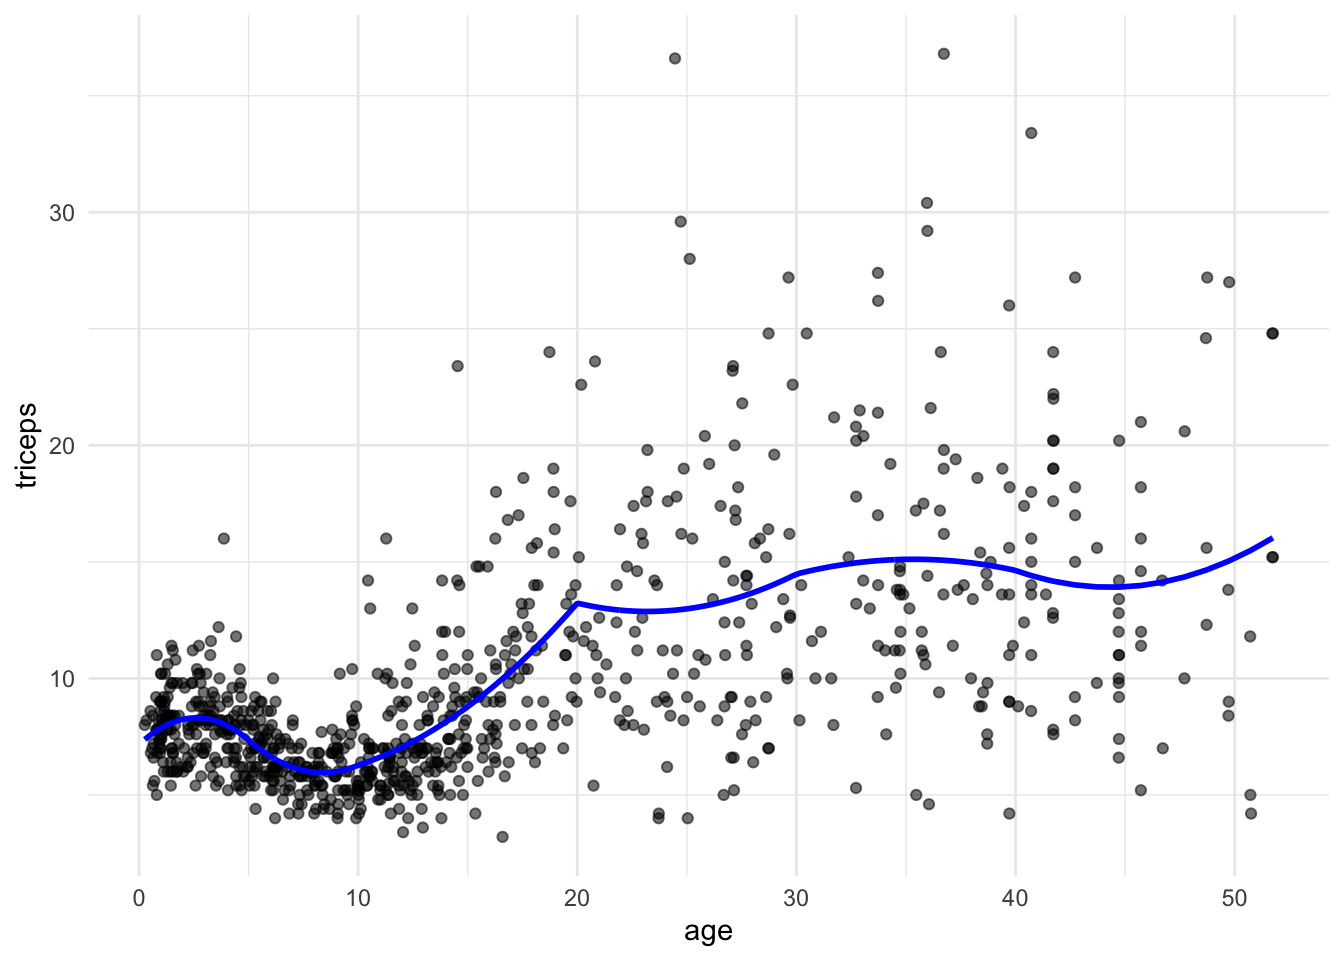
\includegraphics[keepaspectratio]{_main_files/figure-latex/quadpiece-1.pdf}}

\subsection*{Task 2 - Fit a natural cubic spline}\label{task-2---fit-a-natural-cubic-spline}
\addcontentsline{toc}{subsection}{Task 2 - Fit a natural cubic spline}

We will the same dataset \textbf{triceps} as in TASK 1 to fit a natural cubic spline
for the association of \textbf{age} and \textbf{triceps}.

The function \texttt{bs()} in the \texttt{splines} package generates the B-spline basis matrix
for a polynomial spline, and the function \texttt{ns()} in the same library generates
the B-spline basis matrix matrix for a natural cubic spline (restriction that
the fitted curve linear at the extremes). We will compare both.

\begin{Shaded}
\begin{Highlighting}[]
\FunctionTok{library}\NormalTok{(splines)}
\FunctionTok{library}\NormalTok{(MultiKink) }\CommentTok{\#for the data}
\FunctionTok{library}\NormalTok{(ggplot2)   }\CommentTok{\#for the plots}
\FunctionTok{set.seed}\NormalTok{(}\DecValTok{1974}\NormalTok{)     }\CommentTok{\#fix the random generator seed }

\FunctionTok{data}\NormalTok{(}\StringTok{"triceps"}\NormalTok{)   }\CommentTok{\#load the dataset triceps}
                  \CommentTok{\#notice that the variable of interest}
                  \CommentTok{\#it is also called triceps. Don\textquotesingle{}t get }
                  \CommentTok{\#confused!}

\CommentTok{\#linear model with the natural cubic splines function }
\NormalTok{cub.splines.bs }\OtherTok{\textless{}{-}} \FunctionTok{lm}\NormalTok{(triceps }\SpecialCharTok{\textasciitilde{}} \FunctionTok{bs}\NormalTok{(age, }\AttributeTok{knots =} \FunctionTok{c}\NormalTok{(}\DecValTok{5}\NormalTok{,}\DecValTok{10}\NormalTok{,}\DecValTok{20}\NormalTok{,}\DecValTok{30}\NormalTok{,}\DecValTok{40}\NormalTok{)), }
                   \AttributeTok{data=}\NormalTok{triceps)}
\FunctionTok{summary}\NormalTok{(cub.splines.bs)}
\end{Highlighting}
\end{Shaded}

\begin{verbatim}
## 
## Call:
## lm(formula = triceps ~ bs(age, knots = c(5, 10, 20, 30, 40)), 
##     data = triceps)
## 
## Residuals:
##      Min       1Q   Median       3Q      Max 
## -11.5234  -1.6912  -0.2917   1.1356  23.0922 
## 
## Coefficients:
##                                        Estimate Std. Error t value Pr(>|t|)    
## (Intercept)                              6.9598     0.9729   7.154 1.77e-12 ***
## bs(age, knots = c(5, 10, 20, 30, 40))1   2.5367     1.7154   1.479   0.1396    
## bs(age, knots = c(5, 10, 20, 30, 40))2  -0.3032     0.9629  -0.315   0.7529    
## bs(age, knots = c(5, 10, 20, 30, 40))3  -1.9092     1.2993  -1.469   0.1421    
## bs(age, knots = c(5, 10, 20, 30, 40))4   7.4056     1.2179   6.081 1.78e-09 ***
## bs(age, knots = c(5, 10, 20, 30, 40))5   6.1050     1.4043   4.347 1.54e-05 ***
## bs(age, knots = c(5, 10, 20, 30, 40))6  10.1770     1.5427   6.597 7.23e-11 ***
## bs(age, knots = c(5, 10, 20, 30, 40))7   3.9428     1.9082   2.066   0.0391 *  
## bs(age, knots = c(5, 10, 20, 30, 40))8  10.1473     1.7545   5.784 1.01e-08 ***
## ---
## Signif. codes:  0 '***' 0.001 '**' 0.01 '*' 0.05 '.' 0.1 ' ' 1
## 
## Residual standard error: 3.743 on 883 degrees of freedom
## Multiple R-squared:  0.4261, Adjusted R-squared:  0.4209 
## F-statistic: 81.94 on 8 and 883 DF,  p-value: < 2.2e-16
\end{verbatim}

\begin{Shaded}
\begin{Highlighting}[]
\NormalTok{cub.splines.ns }\OtherTok{\textless{}{-}} \FunctionTok{lm}\NormalTok{(triceps }\SpecialCharTok{\textasciitilde{}} \FunctionTok{ns}\NormalTok{(age, }\AttributeTok{knots =} \FunctionTok{c}\NormalTok{(}\DecValTok{5}\NormalTok{,}\DecValTok{10}\NormalTok{,}\DecValTok{20}\NormalTok{,}\DecValTok{30}\NormalTok{,}\DecValTok{40}\NormalTok{)), }
                   \AttributeTok{data=}\NormalTok{triceps)}

\FunctionTok{summary}\NormalTok{(cub.splines.ns)}
\end{Highlighting}
\end{Shaded}

\begin{verbatim}
## 
## Call:
## lm(formula = triceps ~ ns(age, knots = c(5, 10, 20, 30, 40)), 
##     data = triceps)
## 
## Residuals:
##      Min       1Q   Median       3Q      Max 
## -10.4875  -1.6873  -0.3665   1.1146  22.8643 
## 
## Coefficients:
##                                        Estimate Std. Error t value Pr(>|t|)    
## (Intercept)                              8.3811     0.5219  16.059  < 2e-16 ***
## ns(age, knots = c(5, 10, 20, 30, 40))1  -3.5592     0.6712  -5.303 1.44e-07 ***
## ns(age, knots = c(5, 10, 20, 30, 40))2   5.7803     1.0379   5.569 3.39e-08 ***
## ns(age, knots = c(5, 10, 20, 30, 40))3   5.5118     0.9416   5.853 6.78e-09 ***
## ns(age, knots = c(5, 10, 20, 30, 40))4   6.9070     0.9050   7.632 5.99e-14 ***
## ns(age, knots = c(5, 10, 20, 30, 40))5   5.4136     1.3783   3.928 9.24e-05 ***
## ns(age, knots = c(5, 10, 20, 30, 40))6   6.6460     1.0829   6.137 1.27e-09 ***
## ---
## Signif. codes:  0 '***' 0.001 '**' 0.01 '*' 0.05 '.' 0.1 ' ' 1
## 
## Residual standard error: 3.759 on 885 degrees of freedom
## Multiple R-squared:  0.4199, Adjusted R-squared:  0.416 
## F-statistic: 106.8 on 6 and 885 DF,  p-value: < 2.2e-16
\end{verbatim}

Notice that are less regression parameters for the natural spline due to the
linearity restriction. We can see this in the plot. To plot we could either
get predictions from the fitted models or fit the models in the \texttt{ggplot}
function directly:

\begin{Shaded}
\begin{Highlighting}[]
 \CommentTok{\#simple scatter}
\NormalTok{ tri.age.plot }\OtherTok{\textless{}{-}} \FunctionTok{ggplot}\NormalTok{(triceps, }\FunctionTok{aes}\NormalTok{(}\AttributeTok{x=}\NormalTok{age, }\AttributeTok{y=}\NormalTok{triceps)) }\SpecialCharTok{+}
                 \FunctionTok{geom\_point}\NormalTok{(}\AttributeTok{alpha=}\FloatTok{0.55}\NormalTok{, }\AttributeTok{color=}\StringTok{"black"}\NormalTok{) }\SpecialCharTok{+} 
                 \FunctionTok{theme\_minimal}\NormalTok{() }
 
\NormalTok{  tri.age.plot }\SpecialCharTok{+}
    \FunctionTok{stat\_smooth}\NormalTok{(}\AttributeTok{method =} \StringTok{"lm"}\NormalTok{, }
               \AttributeTok{formula =}\NormalTok{ y}\SpecialCharTok{\textasciitilde{}}\FunctionTok{bs}\NormalTok{(x,}\AttributeTok{knots =} \FunctionTok{c}\NormalTok{(}\DecValTok{5}\NormalTok{,}\DecValTok{10}\NormalTok{,}\DecValTok{20}\NormalTok{,}\DecValTok{30}\NormalTok{,}\DecValTok{40}\NormalTok{)), }
               \AttributeTok{lty =} \DecValTok{1}\NormalTok{, }\AttributeTok{col =} \StringTok{"blue"}\NormalTok{) }\SpecialCharTok{+} 
    \FunctionTok{stat\_smooth}\NormalTok{(}\AttributeTok{method =} \StringTok{"lm"}\NormalTok{, }
               \AttributeTok{formula =}\NormalTok{ y}\SpecialCharTok{\textasciitilde{}}\FunctionTok{ns}\NormalTok{(x,}\AttributeTok{knots =} \FunctionTok{c}\NormalTok{(}\DecValTok{5}\NormalTok{,}\DecValTok{10}\NormalTok{,}\DecValTok{20}\NormalTok{,}\DecValTok{30}\NormalTok{,}\DecValTok{40}\NormalTok{)), }
               \AttributeTok{lty =} \DecValTok{1}\NormalTok{, }\AttributeTok{col =} \StringTok{"red"}\NormalTok{)  }
\end{Highlighting}
\end{Shaded}

\pandocbounded{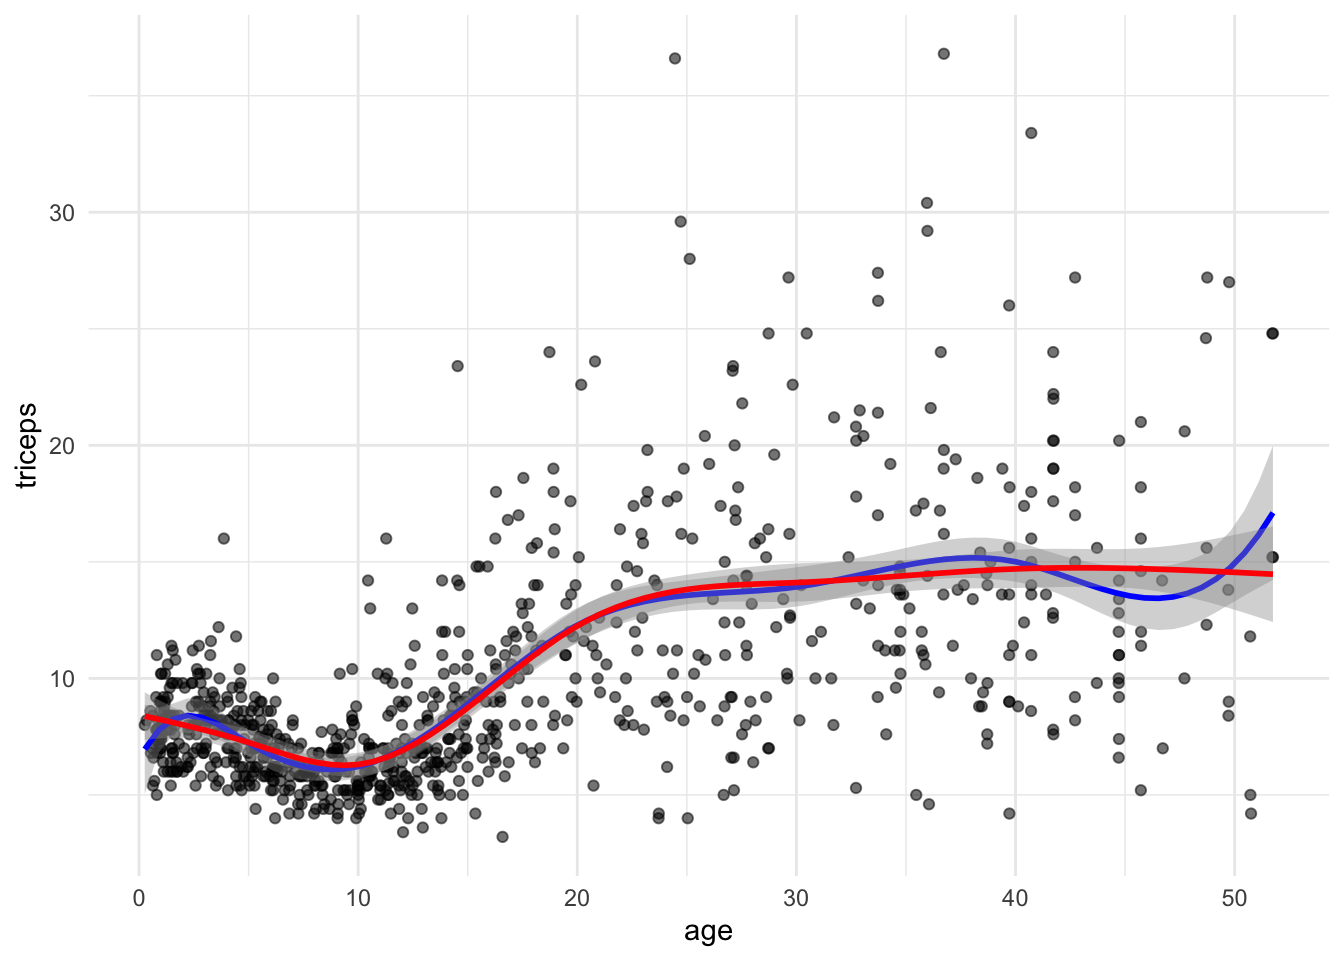
\includegraphics[keepaspectratio]{_main_files/figure-latex/addcubi-1.pdf}}

\textbf{TRY IT YOURSELF:}

\begin{enumerate}
\def\labelenumi{\arabic{enumi})}
\tightlist
\item
  Fit a natural spline with 6 degrees of freedom and compare it with the
  natural spline using \texttt{knots\ =\ c(5,10,20,30,40)}. What is the difference?
\end{enumerate}

See the solution code

\begin{Shaded}
\begin{Highlighting}[]
\NormalTok{ tri.age.plot }\SpecialCharTok{+}
    \FunctionTok{stat\_smooth}\NormalTok{(}\AttributeTok{method =} \StringTok{"lm"}\NormalTok{, }
               \AttributeTok{formula =}\NormalTok{ y}\SpecialCharTok{\textasciitilde{}}\FunctionTok{ns}\NormalTok{(x,}\AttributeTok{knots =} \FunctionTok{c}\NormalTok{(}\DecValTok{5}\NormalTok{,}\DecValTok{10}\NormalTok{,}\DecValTok{20}\NormalTok{,}\DecValTok{30}\NormalTok{,}\DecValTok{40}\NormalTok{)), }
               \AttributeTok{lty =} \DecValTok{1}\NormalTok{, }\AttributeTok{col =} \StringTok{"red"}\NormalTok{) }\SpecialCharTok{+} 
    \FunctionTok{stat\_smooth}\NormalTok{(}\AttributeTok{method =} \StringTok{"lm"}\NormalTok{, }
               \AttributeTok{formula =}\NormalTok{ y}\SpecialCharTok{\textasciitilde{}}\FunctionTok{ns}\NormalTok{(x,}\AttributeTok{df=}\DecValTok{6}\NormalTok{), }
               \AttributeTok{lty =} \DecValTok{1}\NormalTok{, }\AttributeTok{col =} \StringTok{"yellow"}\NormalTok{)      }
\end{Highlighting}
\end{Shaded}

\pandocbounded{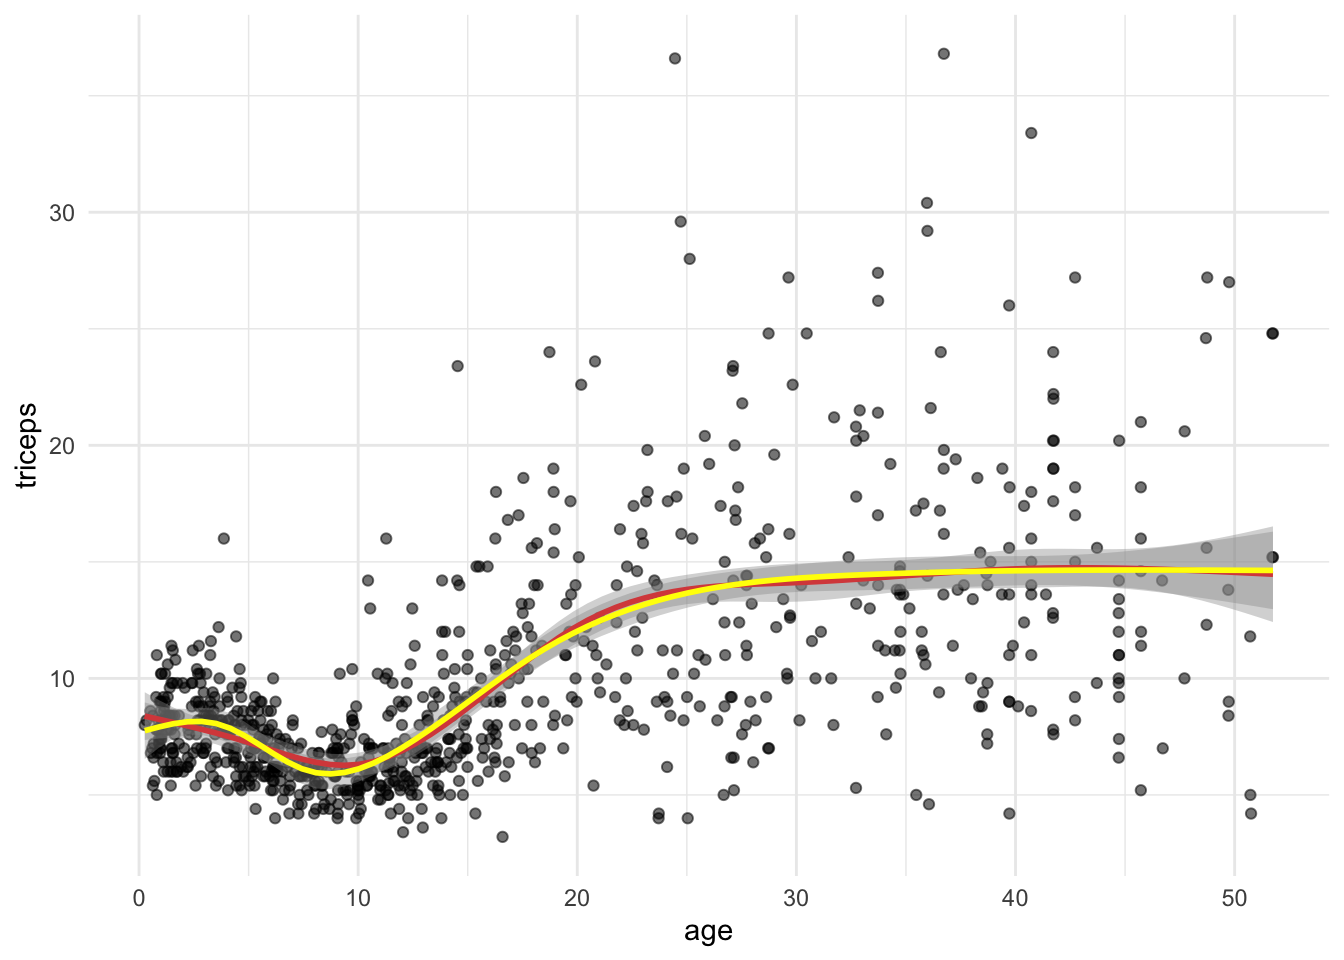
\includegraphics[keepaspectratio]{_main_files/figure-latex/unnamed-chunk-12-1.pdf}}

\begin{Shaded}
\begin{Highlighting}[]
\CommentTok{\#df=6 also chooses 5 knots but the knots}
\CommentTok{\#are based on the quantiles of the data}
\CommentTok{\#in this case the knots are at values:}
\FunctionTok{attr}\NormalTok{(}\FunctionTok{ns}\NormalTok{(triceps}\SpecialCharTok{$}\NormalTok{age, }\AttributeTok{df=}\DecValTok{6}\NormalTok{), }\StringTok{"knots"}\NormalTok{) }
\end{Highlighting}
\end{Shaded}

\begin{verbatim}
## [1]  3.76  7.67 12.21 18.12 32.55
\end{verbatim}

\begin{enumerate}
\def\labelenumi{\arabic{enumi})}
\setcounter{enumi}{1}
\tightlist
\item
  Calculate the MSE (or the root mean squared error) for the models using
  natural cubic splines with \(df\) from 2 (linear model) up to 20. You can use the library \texttt{caret}.
\end{enumerate}

See the solution code

\begin{Shaded}
\begin{Highlighting}[]
\FunctionTok{library}\NormalTok{(caret)}
\FunctionTok{set.seed}\NormalTok{(}\DecValTok{1001}\NormalTok{)}

\CommentTok{\#repeated CV for the MSE}
\NormalTok{trC.lm }\OtherTok{\textless{}{-}} \FunctionTok{trainControl}\NormalTok{(}\AttributeTok{method =} \StringTok{"repeatedcv"}\NormalTok{, }
                         \AttributeTok{number =} \DecValTok{10}\NormalTok{, }
                         \AttributeTok{repeats =} \DecValTok{10}\NormalTok{)}

\CommentTok{\#function to fit a spline with x degrees of freedom}
\NormalTok{  my.spline.f }\OtherTok{\textless{}{-}} \ControlFlowTok{function}\NormalTok{(x) \{}
    \CommentTok{\#need to construct the model formula}
\NormalTok{    spline.formula }\OtherTok{\textless{}{-}} \FunctionTok{as.formula}\NormalTok{(}\FunctionTok{paste}\NormalTok{(}\StringTok{"triceps \textasciitilde{} ns(age, df="}\NormalTok{,x, }\StringTok{")"}\NormalTok{ ))                                          }
\NormalTok{    pol.model }\OtherTok{\textless{}{-}} \FunctionTok{train}\NormalTok{(spline.formula,                   }
                        \AttributeTok{data =}\NormalTok{ triceps,            }
                        \AttributeTok{method =} \StringTok{"lm"}\NormalTok{,}
                        \AttributeTok{trControl =}\NormalTok{ trC.lm)}
    
\NormalTok{    RMSE.cv }\OtherTok{=}\NormalTok{ pol.model}\SpecialCharTok{$}\NormalTok{results[}\DecValTok{2}\NormalTok{]                }\CommentTok{\#extracts the RMSE}
\NormalTok{  \}}
  
  \CommentTok{\#RMSE}
  \FunctionTok{t}\NormalTok{(}\FunctionTok{sapply}\NormalTok{(}\DecValTok{2}\SpecialCharTok{:}\DecValTok{20}\NormalTok{, my.spline.f))                    }\CommentTok{\#Computes the RMSE for splines}
                                                  \CommentTok{\#with df degrees 2 to 20}
  \DocumentationTok{\#\#\#\#\#\#\#\#\#\#\#\#\#\#\#\#\#\#\#\#\#\#\#\#\#\#\#\#\#\#\#\#\#\#\#\#\#\#\#\#\#\#\#\#\#\#\#\#\#\#\#\#\#\#\#\#\#\#\#\#\#\#\#\#\#\#\#\#\#\#\#\#\#\#\#}
  \CommentTok{\#if you want to plot the curves,}
  \CommentTok{\#it is tricky to get ggplot to work }
  \CommentTok{\#within a loop. This is a solutions:}
\NormalTok{  col.ran }\OtherTok{\textless{}{-}} \FunctionTok{sample}\NormalTok{(}\FunctionTok{colours}\NormalTok{(), }\DecValTok{20}\NormalTok{)                  }\CommentTok{\#colours for the lines}
\NormalTok{  my.plot}\OtherTok{\textless{}{-}}\NormalTok{ tri.age.plot                            }\CommentTok{\#scatterplot}
  \ControlFlowTok{for}\NormalTok{ (i }\ControlFlowTok{in} \DecValTok{2}\SpecialCharTok{:}\DecValTok{20}\NormalTok{)\{}
      \CommentTok{\#builds the stat\_smooth with df=i}
\NormalTok{      loop\_input }\OtherTok{\textless{}{-}}  \FunctionTok{paste}\NormalTok{(}\StringTok{"stat\_smooth(method = }\SpecialCharTok{\textbackslash{}"}\StringTok{lm}\SpecialCharTok{\textbackslash{}"}\StringTok{, }
\StringTok{                          formula = y\textasciitilde{}ns(x,df="}\NormalTok{,i,}\StringTok{"), }
\StringTok{                          lty = 1, col =}\SpecialCharTok{\textbackslash{}"}\StringTok{"}\NormalTok{,col.ran[i],}\StringTok{"}\SpecialCharTok{\textbackslash{}"}\StringTok{, }
\StringTok{                          se = FALSE)"}\NormalTok{, }\AttributeTok{sep=}\StringTok{""}\NormalTok{)}
      
      \CommentTok{\#updates the scatter plot with }
      \CommentTok{\#the new spline}
\NormalTok{      my.plot }\OtherTok{\textless{}{-}}\NormalTok{ my.plot }\SpecialCharTok{+} \FunctionTok{eval}\NormalTok{(}\FunctionTok{parse}\NormalTok{(}\AttributeTok{text=}\NormalTok{loop\_input))    }
\NormalTok{  \}}
  
\NormalTok{ my.plot}
\end{Highlighting}
\end{Shaded}

\pandocbounded{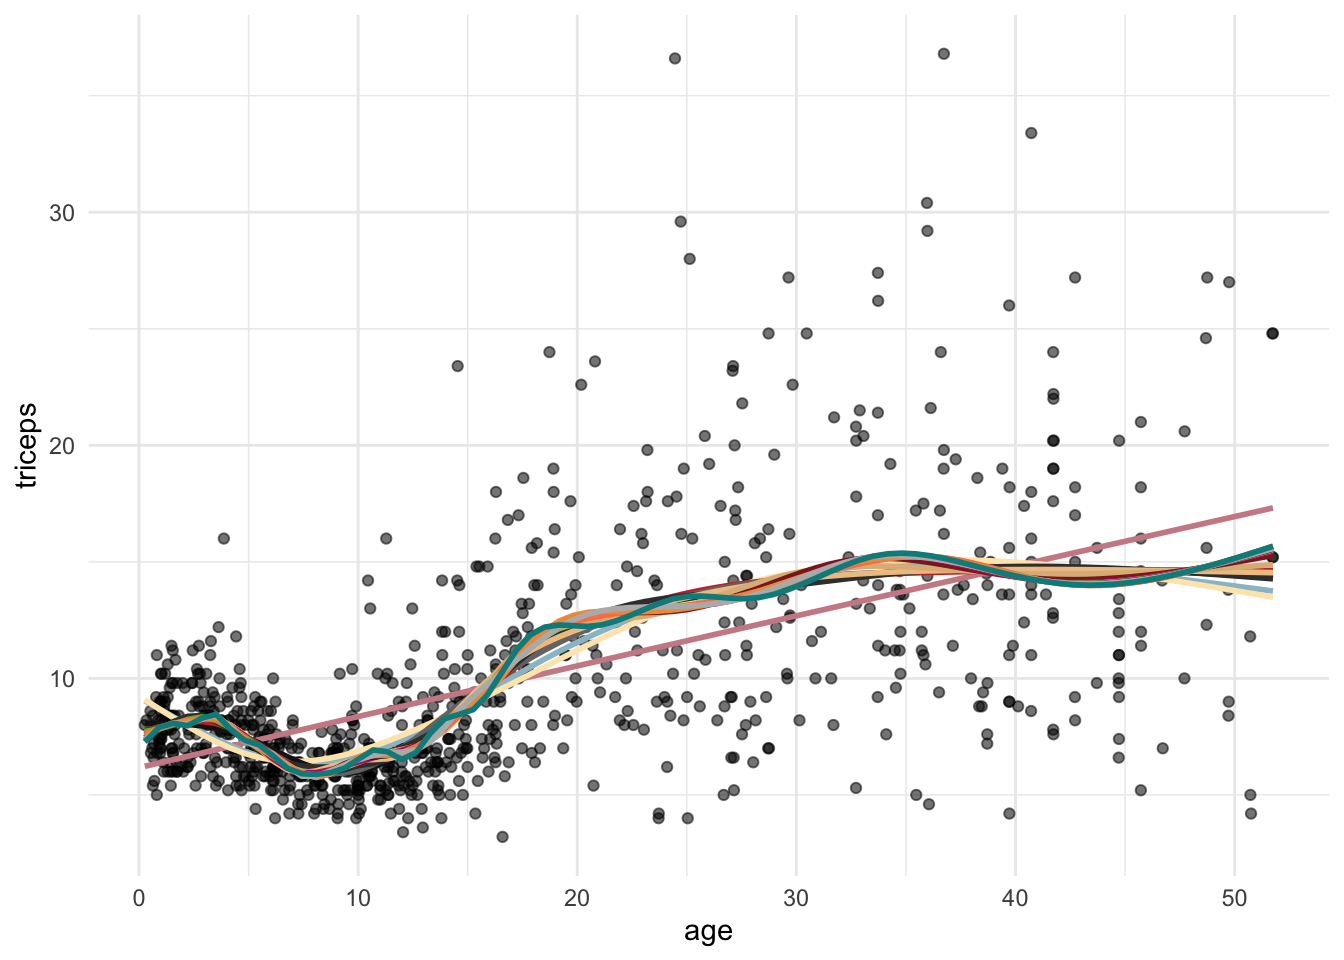
\includegraphics[keepaspectratio]{_main_files/figure-latex/allxplot-1.pdf}}

\section{Exercises}\label{PWR4}

Solve the following exercise:

\begin{enumerate}
\def\labelenumi{\arabic{enumi})}
\tightlist
\item
  The dataset \href{https://www.dropbox.com/s/cwkw3p91zyizcqz/SA_heart.csv?dl=1}{SA\_heart.csv}
  contains on coronary heart disease status (variable \emph{chd}) and several risk
  factors including the cumulative tobacco consumption \emph{tobacco}.
\end{enumerate}

\begin{enumerate}
\def\labelenumi{\alph{enumi})}
\item
  Fit a logistic model for \emph{chd} using the predictor \emph{tobacco}
  (as a linear effect) and compute its AIC
\item
  Plot the fitted curve in a)
\item
  Fit a logistic model for \emph{chd} with a natural cubic spline for the predictor \emph{tobacco}, with \(df\) 5 and 10. Compute the AIC of the two models.
\item
  Plot the fitted curves in c)
\item
  Compute the cross-validated ROC of the models a) and c) (use the \texttt{caret} package)
\end{enumerate}

See the solution code for e)

\begin{Shaded}
\begin{Highlighting}[]
    \FunctionTok{library}\NormalTok{(caret)}
    \FunctionTok{library}\NormalTok{(splines)}
    \FunctionTok{set.seed}\NormalTok{(}\DecValTok{2001}\NormalTok{)}
\NormalTok{    SA\_heart }\OtherTok{\textless{}{-}} \FunctionTok{read.csv}\NormalTok{(}\StringTok{"https://www.dropbox.com/s/cwkw3p91zyizcqz/SA\_heart.csv?dl=1"}\NormalTok{)}
    
    \CommentTok{\# caret will give an error for factors coded as 0 and 1}
    \CommentTok{\# because it uses the factors names to create}
    \CommentTok{\# names of internal variables. This way it is better}
    \CommentTok{\#to use an outcome variable with strings as the factor names}
\NormalTok{    SA\_heart}\SpecialCharTok{$}\NormalTok{chd.f }\OtherTok{\textless{}{-}} \FunctionTok{ifelse}\NormalTok{(SA\_heart}\SpecialCharTok{$}\NormalTok{chd }\SpecialCharTok{==}\DecValTok{1}\NormalTok{, }
                             \StringTok{"chd"}\NormalTok{, }
                             \StringTok{"nochd"}\NormalTok{)     }
    
    \CommentTok{\#sets the control for 10{-}fold cross{-}validation, 10 times}
    \CommentTok{\# the classProbs = TRUE and summaryFunction = twoClassSummary}
    \CommentTok{\# store the information to compute the area under the ROC}
\NormalTok{    trC.lm }\OtherTok{\textless{}{-}} \FunctionTok{trainControl}\NormalTok{(}\AttributeTok{method =} \StringTok{"repeatedcv"}\NormalTok{, }
                           \AttributeTok{number =} \DecValTok{10}\NormalTok{, }
                           \AttributeTok{repeats =} \DecValTok{10}\NormalTok{,}
                           \AttributeTok{classProbs =} \ConstantTok{TRUE}\NormalTok{,                 }\CommentTok{\#necessary for }
                           \AttributeTok{summaryFunction =}\NormalTok{ twoClassSummary) }\CommentTok{\#the AUC ROC}

     \CommentTok{\#linear effect}
\NormalTok{     roc.l }\OtherTok{\textless{}{-}} \FunctionTok{train}\NormalTok{(}\AttributeTok{form =}\NormalTok{ chd.f  }\SpecialCharTok{\textasciitilde{}}\NormalTok{ tobacco,}
                    \AttributeTok{data =}\NormalTok{ SA\_heart,}
                    \AttributeTok{method =} \StringTok{"glm"}\NormalTok{,}
                    \AttributeTok{family =} \StringTok{"binomial"}\NormalTok{,}
                    \AttributeTok{trControl =}\NormalTok{ trC.lm,}
                    \AttributeTok{metric =} \StringTok{"ROC"}\NormalTok{) }
     
\NormalTok{     roc}\FloatTok{.5} \OtherTok{\textless{}{-}} \FunctionTok{train}\NormalTok{(}\AttributeTok{form =}\NormalTok{ chd.f  }\SpecialCharTok{\textasciitilde{}} \FunctionTok{ns}\NormalTok{(tobacco,}\AttributeTok{df=}\DecValTok{5}\NormalTok{),}
                    \AttributeTok{data =}\NormalTok{ SA\_heart,}
                    \AttributeTok{method =} \StringTok{"glm"}\NormalTok{,}
                    \AttributeTok{family =} \StringTok{"binomial"}\NormalTok{,}
                    \AttributeTok{trControl =}\NormalTok{ trC.lm,}
                    \AttributeTok{metric =} \StringTok{"ROC"}\NormalTok{) }
     \CommentTok{\#cubic effect}
\NormalTok{     roc}\FloatTok{.10} \OtherTok{\textless{}{-}} \FunctionTok{train}\NormalTok{(}\AttributeTok{form =}\NormalTok{ chd.f  }\SpecialCharTok{\textasciitilde{}} \FunctionTok{ns}\NormalTok{(tobacco,}\AttributeTok{df=}\DecValTok{10}\NormalTok{),}
                    \AttributeTok{data =}\NormalTok{ SA\_heart,}
                    \AttributeTok{method =} \StringTok{"glm"}\NormalTok{,}
                    \AttributeTok{family =} \StringTok{"binomial"}\NormalTok{,}
                    \AttributeTok{trControl =}\NormalTok{ trC.lm,}
                    \AttributeTok{metric =} \StringTok{"ROC"}\NormalTok{) }
  
\NormalTok{     roc.l}
\NormalTok{     roc}\FloatTok{.5}
\NormalTok{     roc}\FloatTok{.10}
\end{Highlighting}
\end{Shaded}

\begin{enumerate}
\def\labelenumi{\alph{enumi})}
\setcounter{enumi}{5}
\tightlist
\item
  Which model would you prefer?
\end{enumerate}

\begin{enumerate}
\def\labelenumi{\arabic{enumi})}
\setcounter{enumi}{1}
\tightlist
\item
  The dataset \href{https://www.dropbox.com/s/jeqdtq04zl9f0er/FEV.csv?dl=1}{fev.csv} contains the measurements of forced expiratory volume (FEV) tests, evaluating the pulmonary capacity in 654 children and young adults.
\end{enumerate}

\begin{enumerate}
\def\labelenumi{\alph{enumi})}
\item
  Plot the association between \emph{fev} and \emph{height} and fit a linear model for \emph{fev} using \emph{height} as a predictor
\item
  Fit a model for \emph{fev} with a cubic b-spline for the predictor \emph{height}, with \(df\) 5 and 10.
\item
  Fit a model for \emph{fev} with a natural cubin spline for the predictor \emph{height}, with \(df\) 5 and 10.
\item
  Plot the fitted curves for models a), b) and c)
\item
  compare the cross-validated MSE of the models a), b) and c)
\end{enumerate}

\chapter{Smoothing splines}\label{smoothing-splines}

\section{Introduction}\label{SS1}

In the previous section we learn how to fit regression splines by specifying
the knots and a set of basis function. It should be easy to see that a higher
number of knots will lead to a lower MSE because we will be overfitting the
features of the curve.

The model below is fitted with natural splines with 25 knots.

\pandocbounded{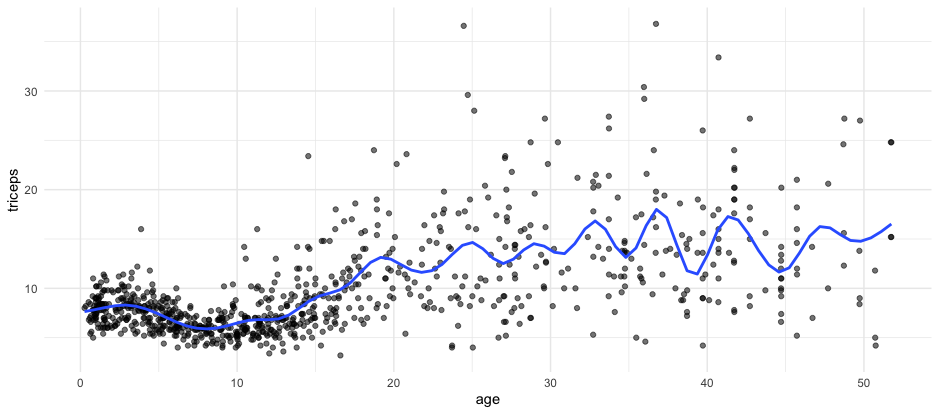
\includegraphics[keepaspectratio]{module4_3_manyknots.png}}
Clearly the curve seems to be overfitting the data.

We will use a similar idea to the one used in regularisation (module 4). We
select many knots but penalise for the roughness of the fitting.

Remember that
the 1st derivative indicates the slope of the curve and the second derivative
is the speed of change of the slope. Thus, the second derivative of a curve is
associated with the roughness of the curve.

We will then use the second derivative as the penalisation term in the
residual sum of squares.

\(\sum_{i=1}^{n} (y_i-f(x_i))^2 + \lambda \int f''(t)^2 dt\)

The result is a \textbf{smoothing spline}. For smoothing splines, the number
of knots is not as important given that the penalisation
term will handle the roughness.

The animation below, shows the fitting of smoothing splines, with
amounts of penalisation (\emph{lambda}), and automatic choice of number of knots
given by the \texttt{smooth.spline} function in R. The cross validated MSE is also
shown.

A large \(\lambda\) results in a smooth curve (a straight line in the limit)
and a smaller \(\lambda\) leads to a more rough curve. The optimal \(\lambda\)
can be chosen by cross-validation.

The smoothing splines can be incorporated in the generalised linear models
framework which is usually referred as \textbf{generalised additive models} (GAM).
Rather than a linear effect of a predictor, we can have a smoothing spline
modeling
the association of the predictor with the outcome:

\(g\left(E(y|\mathbf{x} ) \right) = \beta_0 + f_1(x_{1}) + f_2(x_{2}) + ... + f_k(x_{k})\)

Notice that \(f_p(x_p)\) can be a linear function \(\beta_p x_p\) and if all \(f\)'s
are linear function, the model above is a GLM.

\section{Readings}\label{SS2}

Read the following chapters of \emph{An introduction to statistical learning}:

\begin{itemize}
\tightlist
\item
  7.5 Smoothing Splines
\item
  7.7 Generalised Additive Model
\end{itemize}

\section{Practice session}\label{SS3}

\subsection*{Task 1 - Fit a smoothing spline}\label{task-1---fit-a-smoothing-spline}
\addcontentsline{toc}{subsection}{Task 1 - Fit a smoothing spline}

We will continue the example using the dataset \textbf{triceps}available in
the \texttt{MultiKink} package. The data contains the measurement of the triceps
skin fold of 892 females (variable \emph{triceps}) and we want to model
its association with \textbf{age}, using smoothing cubic splines.

The function \texttt{smooth.spline()} fits smoothing cubic splines. We can provide the
penalisation and/or number of knots, df, or just use the defaults.

\begin{Shaded}
\begin{Highlighting}[]
\FunctionTok{library}\NormalTok{(splines)}
\FunctionTok{library}\NormalTok{(MultiKink) }\CommentTok{\#for the data}
\FunctionTok{library}\NormalTok{(ggplot2)   }\CommentTok{\#for the plots}
\FunctionTok{set.seed}\NormalTok{(}\DecValTok{1974}\NormalTok{)     }\CommentTok{\#fix the random generator seed }

\FunctionTok{data}\NormalTok{(}\StringTok{"triceps"}\NormalTok{)   }\CommentTok{\#load the dataset triceps}
                  \CommentTok{\#notice that the variable of interest}
                  \CommentTok{\#it is also called triceps. Don\textquotesingle{}t get }
                  \CommentTok{\#confused!}

\CommentTok{\#smooth spline with automatic number of knots chosen}
\CommentTok{\#and penalisation chosen by leave{-}one{-}out CV (this is the}
\CommentTok{\#option cv=T, otherwise generalized’ cross{-}validation is used)}
\NormalTok{sspline }\OtherTok{\textless{}{-}} \FunctionTok{smooth.spline}\NormalTok{(triceps}\SpecialCharTok{$}\NormalTok{age, }
\NormalTok{                         triceps}\SpecialCharTok{$}\NormalTok{triceps, }
                         \AttributeTok{cv=}\ConstantTok{TRUE}\NormalTok{) }
\end{Highlighting}
\end{Shaded}

\begin{verbatim}
## Warning in smooth.spline(triceps$age, triceps$triceps, cv = TRUE):
## cross-validation with non-unique 'x' values seems doubtful
\end{verbatim}

\begin{Shaded}
\begin{Highlighting}[]
\FunctionTok{plot}\NormalTok{(triceps}\SpecialCharTok{$}\NormalTok{age, triceps}\SpecialCharTok{$}\NormalTok{triceps)}
\FunctionTok{lines}\NormalTok{(sspline, }\AttributeTok{col=}\StringTok{"blue"}\NormalTok{)}
\end{Highlighting}
\end{Shaded}

\pandocbounded{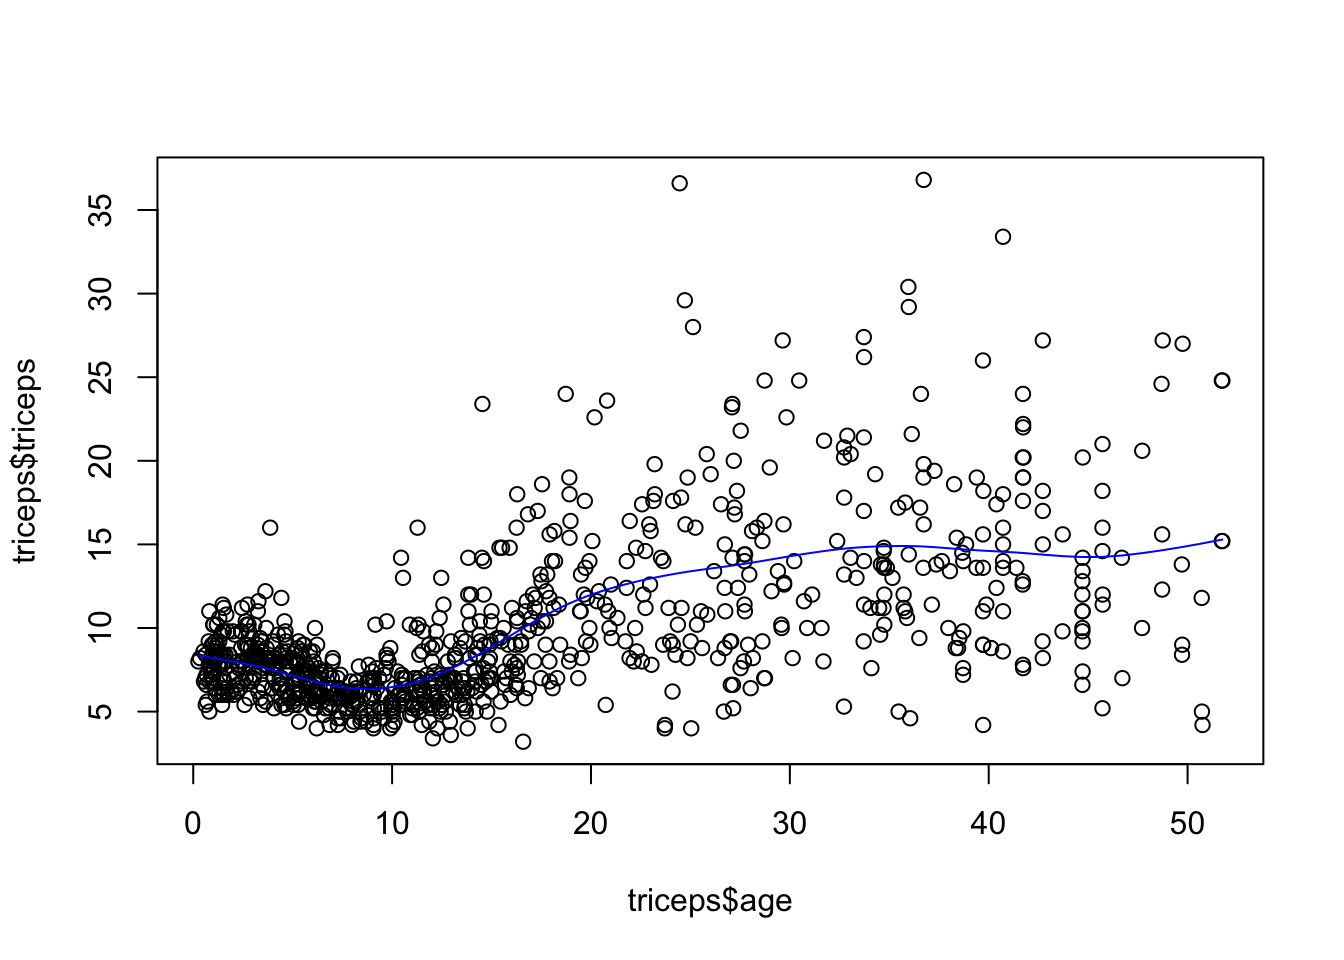
\includegraphics[keepaspectratio]{_main_files/figure-latex/unnamed-chunk-14-1.pdf}}

*Note: The generalised cross-validation (default), in this case, selects a
very low value for \(\lambda\) which results in under smoothing. It is not clear
why that is the case.

Let's get the triceps predicted value for the ages of 10 and 30

\begin{Shaded}
\begin{Highlighting}[]
\FunctionTok{predict}\NormalTok{(sspline, }\AttributeTok{x=}\FunctionTok{c}\NormalTok{(}\DecValTok{10}\NormalTok{,}\DecValTok{30}\NormalTok{))}
\end{Highlighting}
\end{Shaded}

\begin{verbatim}
## $x
## [1] 10 30
## 
## $y
## [1]  6.470573 14.290032
\end{verbatim}

The predicted values are 6.4705727 and
14.2900322, respectively.

As mentioned before, we could have chosen the amount of penalisation and this
would lead to a different smoothing. For example, for

\begin{Shaded}
\begin{Highlighting}[]
\NormalTok{sspline }\OtherTok{\textless{}{-}} \FunctionTok{smooth.spline}\NormalTok{(triceps}\SpecialCharTok{$}\NormalTok{age, }
\NormalTok{                         triceps}\SpecialCharTok{$}\NormalTok{triceps, }\AttributeTok{lambda=}\NormalTok{.}\DecValTok{0001}\NormalTok{) }
\FunctionTok{plot}\NormalTok{(triceps}\SpecialCharTok{$}\NormalTok{age, triceps}\SpecialCharTok{$}\NormalTok{triceps)}
\FunctionTok{lines}\NormalTok{(sspline, }\AttributeTok{col=}\StringTok{"blue"}\NormalTok{)}
\end{Highlighting}
\end{Shaded}

\pandocbounded{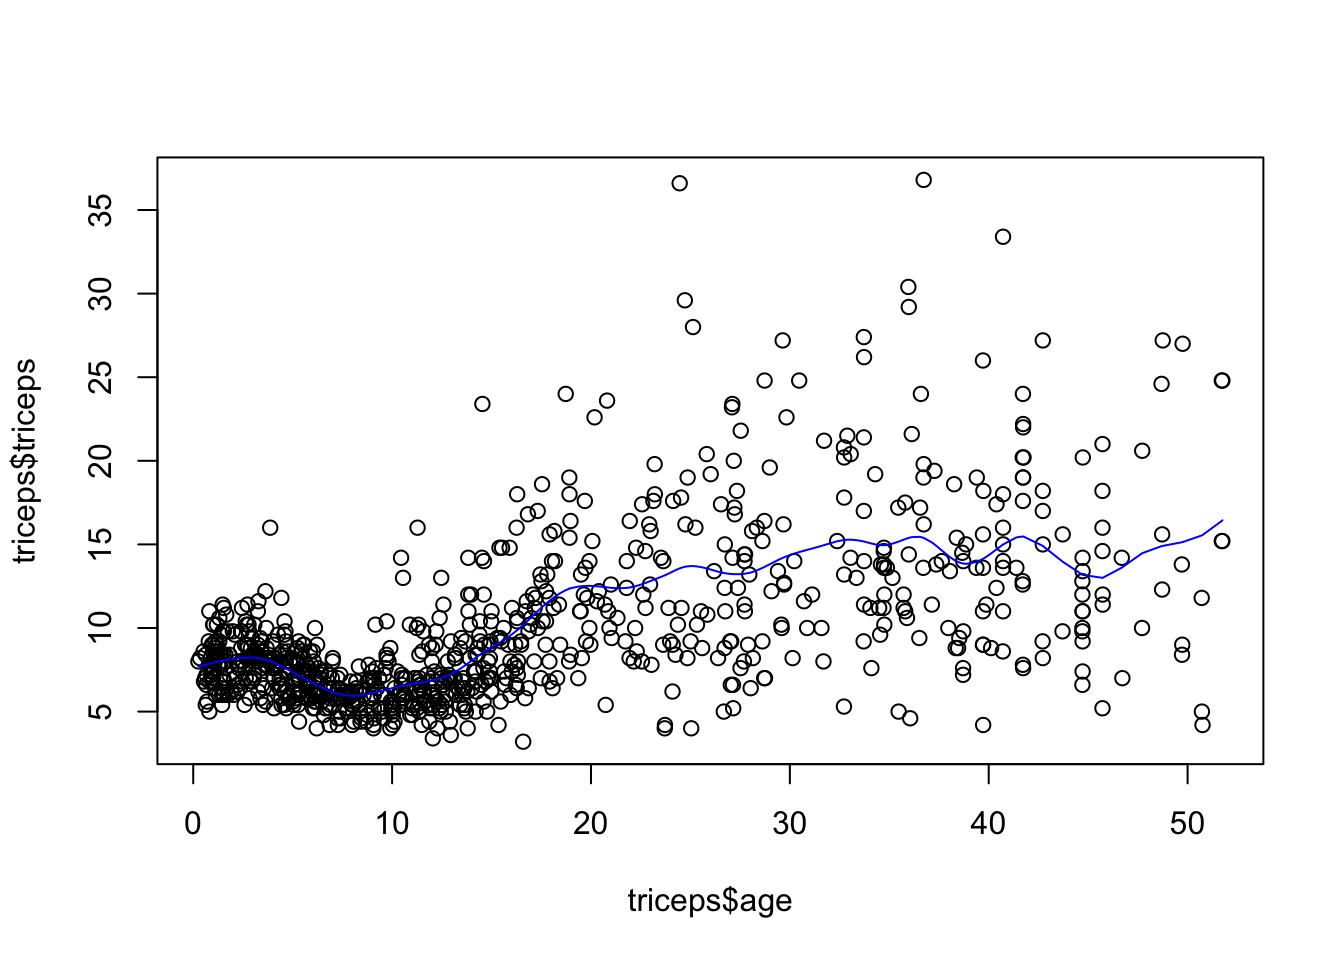
\includegraphics[keepaspectratio]{_main_files/figure-latex/unnamed-chunk-16-1.pdf}}

\textbf{TRY IT YOURSELF:}

\begin{enumerate}
\def\labelenumi{\arabic{enumi})}
\tightlist
\item
  Fit smoothing splines with \emph{df=19} and \emph{df=30} and compare them with the one
  above. Comment on the results.
\end{enumerate}

See the solution code

\begin{Shaded}
\begin{Highlighting}[]
\NormalTok{sspline }\OtherTok{\textless{}{-}} \FunctionTok{smooth.spline}\NormalTok{(triceps}\SpecialCharTok{$}\NormalTok{age, }
\NormalTok{                         triceps}\SpecialCharTok{$}\NormalTok{triceps, }\AttributeTok{lambda=}\NormalTok{.}\DecValTok{0001}\NormalTok{) }
\NormalTok{sspline19 }\OtherTok{\textless{}{-}} \FunctionTok{smooth.spline}\NormalTok{(triceps}\SpecialCharTok{$}\NormalTok{age, }
\NormalTok{                         triceps}\SpecialCharTok{$}\NormalTok{triceps, }\AttributeTok{df=}\DecValTok{19}\NormalTok{) }
\NormalTok{sspline30 }\OtherTok{\textless{}{-}} \FunctionTok{smooth.spline}\NormalTok{(triceps}\SpecialCharTok{$}\NormalTok{age, }
\NormalTok{                         triceps}\SpecialCharTok{$}\NormalTok{triceps, }\AttributeTok{df=}\DecValTok{30}\NormalTok{) }
\FunctionTok{plot}\NormalTok{(triceps}\SpecialCharTok{$}\NormalTok{age, triceps}\SpecialCharTok{$}\NormalTok{triceps)}
\FunctionTok{lines}\NormalTok{(sspline, }\AttributeTok{col=}\StringTok{"blue"}\NormalTok{)}
\FunctionTok{lines}\NormalTok{(sspline19, }\AttributeTok{col=}\StringTok{"red"}\NormalTok{)}
\FunctionTok{lines}\NormalTok{(sspline30, }\AttributeTok{col=}\StringTok{"green"}\NormalTok{)}
\end{Highlighting}
\end{Shaded}

\pandocbounded{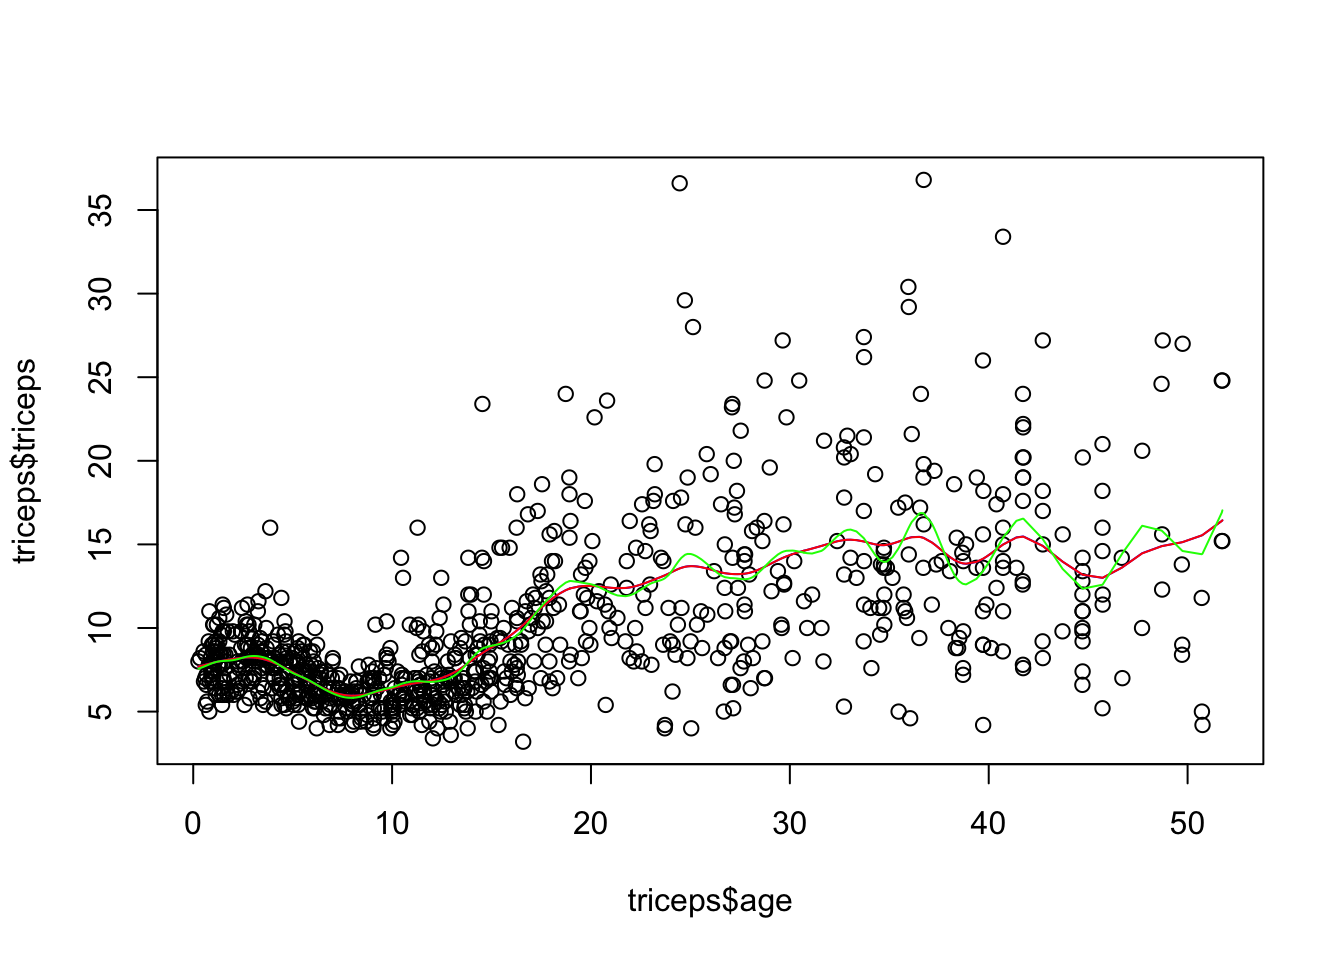
\includegraphics[keepaspectratio]{_main_files/figure-latex/unnamed-chunk-17-1.pdf}}

The spline with df=19 corresponds to having a lambda=.0001, so the result is the
same. If you run \texttt{sspline} and \texttt{sspline} you can see that the parameters are
similar.

The spline with df=30 will be more flexible (more rough).

\subsection*{Task 2 - Fit an additive model}\label{task-2---fit-an-additive-model}
\addcontentsline{toc}{subsection}{Task 2 - Fit an additive model}

The dataset \href{https://www.dropbox.com/s/7wjsfdaf0wt2kg2/bmd.csv?dl=1}{bmd.csv}
contains 169 measurement of bone mineral density (variable \emph{bmd}) in men and
women of different age. We want to fit a model for \emph{bmd} using \emph{age}, \emph{sex}
and \emph{bmi} as predictors.

\begin{Shaded}
\begin{Highlighting}[]
\CommentTok{\#read the data and compute BMI}
\NormalTok{bmd.data     }\OtherTok{\textless{}{-}} 
  \FunctionTok{read.csv}\NormalTok{(}\StringTok{"https://www.dropbox.com/s/c6mhgatkotuze8o/bmd.csv?dl=1"}\NormalTok{, }
           \AttributeTok{stringsAsFactors =} \ConstantTok{TRUE}\NormalTok{)}
\NormalTok{bmd.data}\SpecialCharTok{$}\NormalTok{bmi }\OtherTok{\textless{}{-}}\NormalTok{ bmd.data}\SpecialCharTok{$}\NormalTok{weight\_kg }\SpecialCharTok{/}\NormalTok{ (bmd.data}\SpecialCharTok{$}\NormalTok{height\_cm}\SpecialCharTok{/}\DecValTok{100}\NormalTok{)}\SpecialCharTok{\^{}}\DecValTok{2}
\end{Highlighting}
\end{Shaded}

We will use the function \texttt{gam()} from the \texttt{mgcv} library. Notice that there is
another gam function from the gam package (from the help file: ``Note that this version of gam is different from the function with the same name in the R library mgcv, which uses only smoothing splines with a focus on automatic smoothing parameter selection via GCV.'')

The function \texttt{s()} within the model indicates that we want to smoothing spline
for that predictor. There are several types of splines implemented in the
function. We will use the option basis spline equal to cubic regression splines:
\texttt{bs="cr"}. The function \texttt{s()} has similarities to the \texttt{smooth.spline()} but
is implemented

\begin{Shaded}
\begin{Highlighting}[]
\CommentTok{\#libraries that we will need}
\FunctionTok{library}\NormalTok{(mgcv)   }\CommentTok{\#package for gam}
\FunctionTok{set.seed}\NormalTok{(}\DecValTok{1974}\NormalTok{) }\CommentTok{\#fix the random generator seed }
\NormalTok{bmd.gam }\OtherTok{\textless{}{-}} \FunctionTok{gam}\NormalTok{(bmd }\SpecialCharTok{\textasciitilde{}} \FunctionTok{s}\NormalTok{(age, }\AttributeTok{bs=}\StringTok{"cr"}\NormalTok{)}\SpecialCharTok{+} \FunctionTok{s}\NormalTok{(bmi, }\AttributeTok{bs=}\StringTok{"cr"}\NormalTok{) }\SpecialCharTok{+}\NormalTok{ sex, }\AttributeTok{data=}\NormalTok{bmd.data)}

\FunctionTok{summary}\NormalTok{(bmd.gam)}
\end{Highlighting}
\end{Shaded}

\begin{verbatim}
## 
## Family: gaussian 
## Link function: identity 
## 
## Formula:
## bmd ~ s(age, bs = "cr") + s(bmi, bs = "cr") + sex
## 
## Parametric coefficients:
##             Estimate Std. Error t value Pr(>|t|)    
## (Intercept)  0.74193    0.01456   50.97  < 2e-16 ***
## sexM         0.08092    0.02064    3.92 0.000131 ***
## ---
## Signif. codes:  0 '***' 0.001 '**' 0.01 '*' 0.05 '.' 0.1 ' ' 1
## 
## Approximate significance of smooth terms:
##          edf Ref.df     F  p-value    
## s(age) 1.035  1.070 17.65 3.02e-05 ***
## s(bmi) 5.687  6.611 10.09  < 2e-16 ***
## ---
## Signif. codes:  0 '***' 0.001 '**' 0.01 '*' 0.05 '.' 0.1 ' ' 1
## 
## R-sq.(adj) =  0.381   Deviance explained = 40.9%
## GCV = 0.018099  Scale est. = 0.017165  n = 169
\end{verbatim}

The effective number of degrees of freedom for age is approximately 1, which
suggests that the effect of age is linear. We can plot the fitted splines
for each predictor. Notice, however, that the plot is not in the original scale.

\begin{Shaded}
\begin{Highlighting}[]
\FunctionTok{plot}\NormalTok{(bmd.gam)}
\end{Highlighting}
\end{Shaded}

\pandocbounded{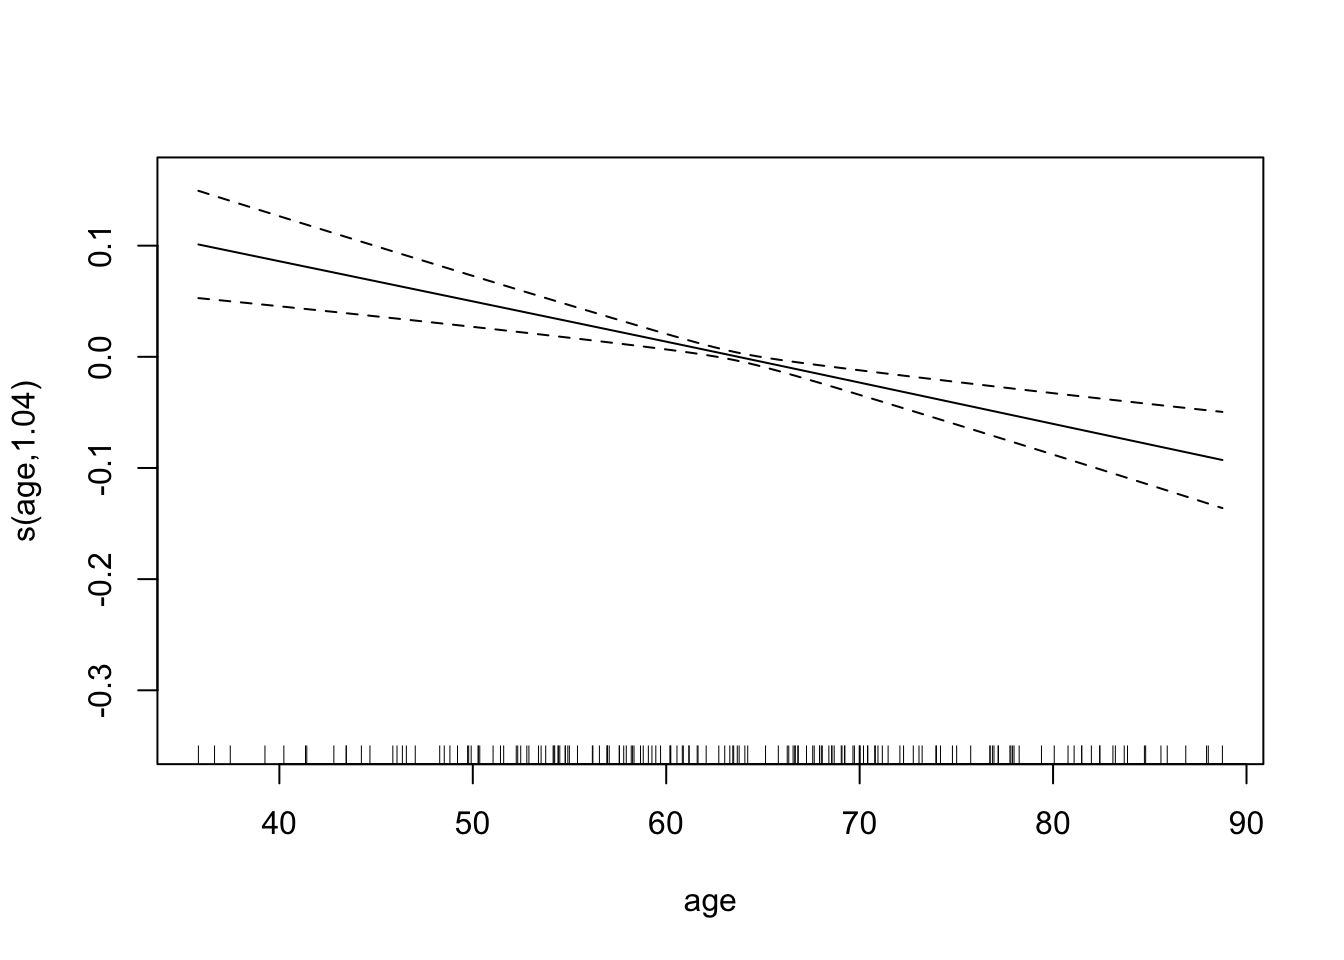
\includegraphics[keepaspectratio]{_main_files/figure-latex/plotgam-1.pdf}} \pandocbounded{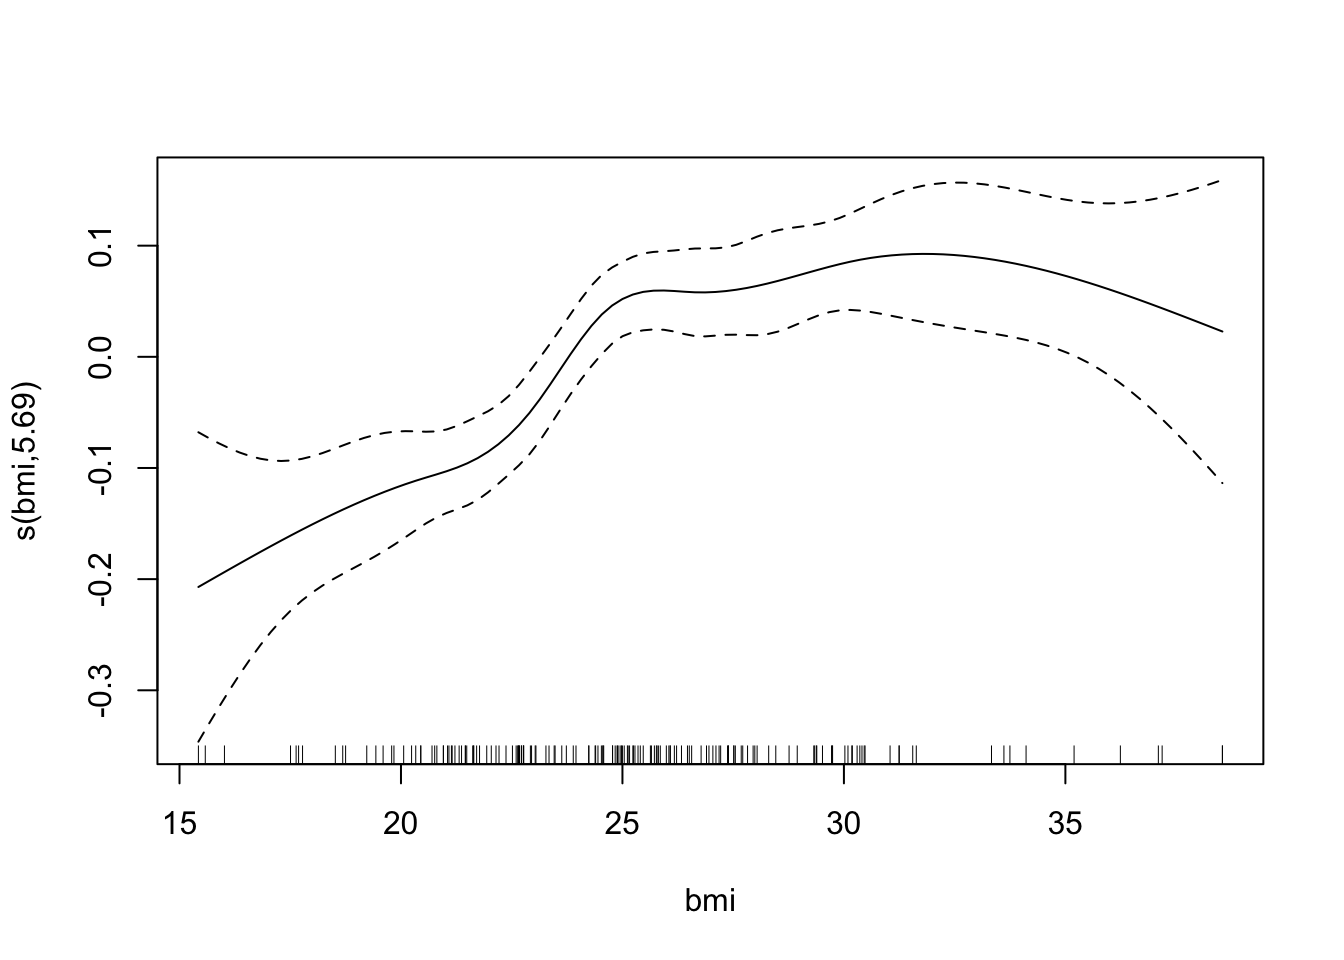
\includegraphics[keepaspectratio]{_main_files/figure-latex/plotgam-2.pdf}}

We can also plot the surface fitted for each sex. For example, for women,

\begin{Shaded}
\begin{Highlighting}[]
\CommentTok{\# Let\textquotesingle{}s create a grid to be used in  persp() }
\NormalTok{steps }\OtherTok{\textless{}{-}} \DecValTok{60}
\NormalTok{age }\OtherTok{\textless{}{-}} \FunctionTok{with}\NormalTok{(bmd.data, }
            \FunctionTok{seq}\NormalTok{(}\FunctionTok{min}\NormalTok{(age), }\FunctionTok{max}\NormalTok{(age), }
                \AttributeTok{length =}\NormalTok{ steps) )}

\NormalTok{bmi }\OtherTok{\textless{}{-}}  \FunctionTok{with}\NormalTok{(bmd.data, }
             \FunctionTok{seq}\NormalTok{(}\FunctionTok{min}\NormalTok{(bmi), }\FunctionTok{max}\NormalTok{(bmi), }
                 \AttributeTok{length =}\NormalTok{ steps) )}

\NormalTok{newdat }\OtherTok{\textless{}{-}} \FunctionTok{expand.grid}\NormalTok{(}\AttributeTok{age =}\NormalTok{ age,             }\CommentTok{\#grid}
                      \AttributeTok{bmi =}\NormalTok{ bmi, }
                      \AttributeTok{sex=}\StringTok{"F"}\NormalTok{)  }

\NormalTok{bmdpred }\OtherTok{\textless{}{-}} \FunctionTok{matrix}\NormalTok{(}\FunctionTok{predict}\NormalTok{(bmd.gam, newdat), }
\NormalTok{                  steps, steps)             }\CommentTok{\#predictions}

\CommentTok{\# Now plot it}
\NormalTok{p }\OtherTok{\textless{}{-}} \FunctionTok{persp}\NormalTok{(age, bmi,}
\NormalTok{           bmdpred, }
           \AttributeTok{theta =} \DecValTok{65}\NormalTok{,                    }\CommentTok{\#angle of the perspective}
           \AttributeTok{col =} \StringTok{"green"}\NormalTok{)}

\CommentTok{\# To add the points, you need the same 3d transformation}
\NormalTok{obs }\OtherTok{\textless{}{-}} \FunctionTok{with}\NormalTok{(bmd.data[bmd.data}\SpecialCharTok{$}\NormalTok{sex}\SpecialCharTok{==}\StringTok{"F"}\NormalTok{, ], }
            \FunctionTok{trans3d}\NormalTok{(age, bmi, bmd, p))}
\NormalTok{pred }\OtherTok{\textless{}{-}} \FunctionTok{with}\NormalTok{(bmd.data[bmd.data}\SpecialCharTok{$}\NormalTok{sex}\SpecialCharTok{==}\StringTok{"F"}\NormalTok{, ], }
             \FunctionTok{trans3d}\NormalTok{(age, bmi, }\FunctionTok{fitted}\NormalTok{(bmd.gam)[bmd.data}\SpecialCharTok{$}\NormalTok{sex}\SpecialCharTok{==}\StringTok{"F"}\NormalTok{], p))}


\CommentTok{\# Add segments to show the points and where they are in 3d}
\FunctionTok{points}\NormalTok{(obs, }\AttributeTok{col =} \StringTok{"red"}\NormalTok{, }\AttributeTok{pch =} \DecValTok{16}\NormalTok{)}
\FunctionTok{segments}\NormalTok{(obs}\SpecialCharTok{$}\NormalTok{x, obs}\SpecialCharTok{$}\NormalTok{y, pred}\SpecialCharTok{$}\NormalTok{x, pred}\SpecialCharTok{$}\NormalTok{y)}
\end{Highlighting}
\end{Shaded}

\pandocbounded{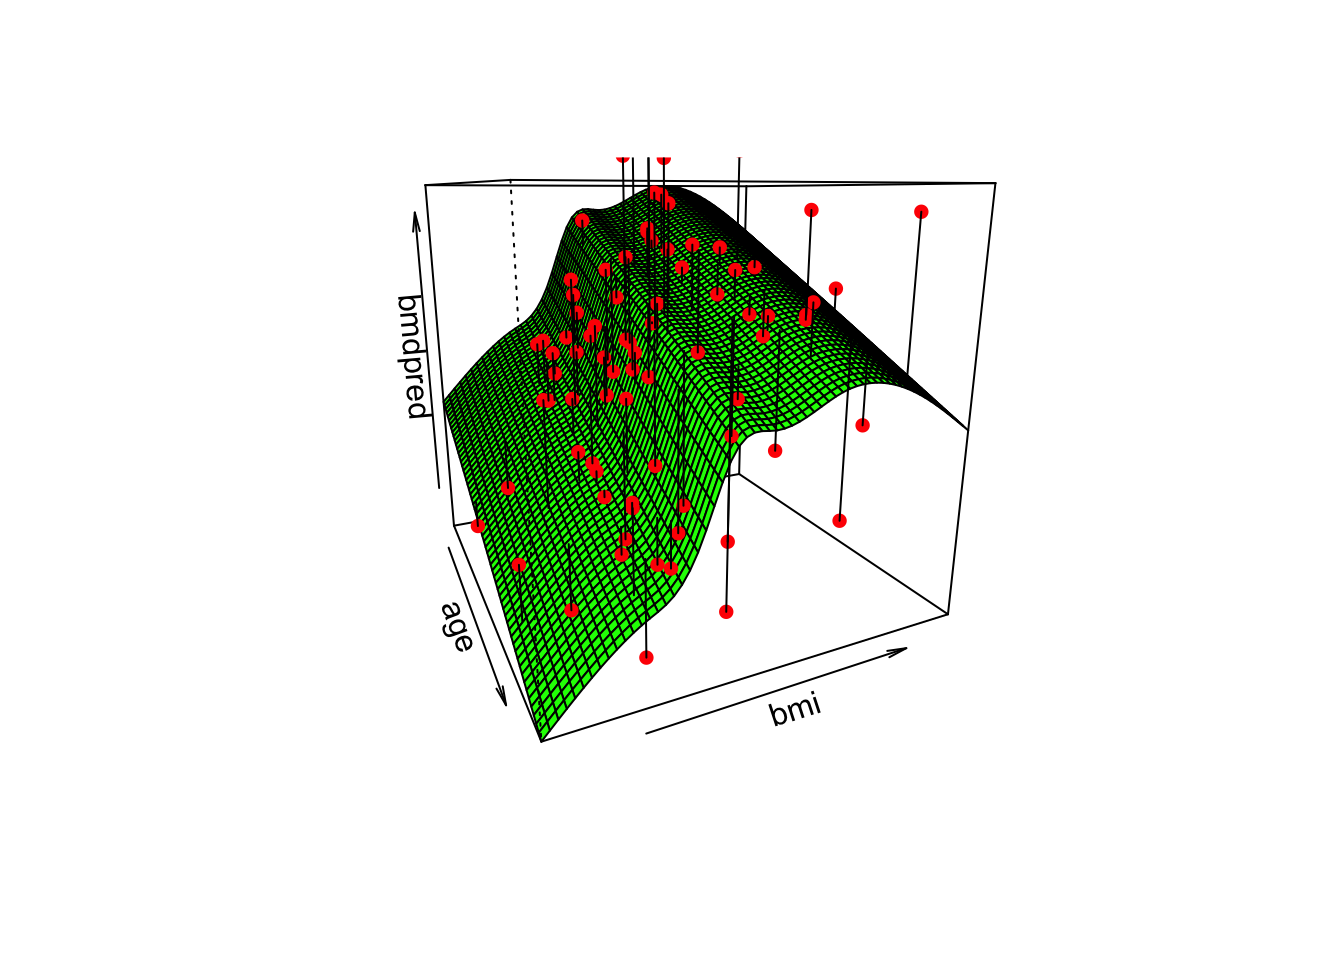
\includegraphics[keepaspectratio]{_main_files/figure-latex/unnamed-chunk-20-1.pdf}}

\textbf{TRY IT YOURSELF:}

\begin{enumerate}
\def\labelenumi{\arabic{enumi})}
\tightlist
\item
  How would the plot for sex=M compare to the surface above?
\end{enumerate}

See the solution code

The surface would have exactly the same shape but would be separated by the 0.08
units (estimate for the variable sex in the model)

\begin{enumerate}
\def\labelenumi{\arabic{enumi})}
\setcounter{enumi}{1}
\tightlist
\item
  Fit a linear model with the same variables and compare the AIC of the linear
  model with the previous GAM model
\end{enumerate}

See the solution code

\begin{Shaded}
\begin{Highlighting}[]
\NormalTok{bmd.glm }\OtherTok{\textless{}{-}} \FunctionTok{glm}\NormalTok{(bmd }\SpecialCharTok{\textasciitilde{}}\NormalTok{ age}\SpecialCharTok{+}\NormalTok{bmi}\SpecialCharTok{+}\NormalTok{ sex, }\AttributeTok{data=}\NormalTok{bmd.data)}
\FunctionTok{summary}\NormalTok{(bmd.glm)}
\FunctionTok{AIC}\NormalTok{(bmd.glm, bmd.gam)}
\end{Highlighting}
\end{Shaded}

The GAM model seems to fit better because it has a lower AIC.

\section{Exercises}\label{SS4}

Solve the following exercise:

\begin{enumerate}
\def\labelenumi{\arabic{enumi})}
\tightlist
\item
  The dataset \href{https://www.dropbox.com/s/cwkw3p91zyizcqz/SA_heart.csv?dl=1}{SA\_heart.csv}
  contains on coronary heart disease status (variable \emph{chd}) and several risk
  factors including the cumulative tobacco consumption \emph{tobacco}, systolic \emph{sbp},
  and \emph{age}
\end{enumerate}

\begin{enumerate}
\def\labelenumi{\alph{enumi})}
\tightlist
\item
  Fit a GAM logistic model for \emph{chd} with splines for the predictor
  \emph{tobacco},\emph{sbp} and \emph{age}
\end{enumerate}

See the solution code for a)

\begin{Shaded}
\begin{Highlighting}[]
    \FunctionTok{library}\NormalTok{(caret)}
    \FunctionTok{library}\NormalTok{(splines)}
    \FunctionTok{set.seed}\NormalTok{(}\DecValTok{2001}\NormalTok{)}
\NormalTok{    SA\_heart }\OtherTok{\textless{}{-}} \FunctionTok{read.csv}\NormalTok{(}\StringTok{"https://www.dropbox.com/s/cwkw3p91zyizcqz/SA\_heart.csv?dl=1"}\NormalTok{)}
    
\NormalTok{    chd.gam }\OtherTok{\textless{}{-}} \FunctionTok{gam}\NormalTok{(chd }\SpecialCharTok{\textasciitilde{}} \FunctionTok{s}\NormalTok{(tobacco, }\AttributeTok{bs=}\StringTok{"cr"}\NormalTok{) }\SpecialCharTok{+} 
                     \FunctionTok{s}\NormalTok{(sbp, }\AttributeTok{bs=}\StringTok{"cr"}\NormalTok{) }\SpecialCharTok{+}
                     \FunctionTok{s}\NormalTok{(age, }\AttributeTok{bs=}\StringTok{"cr"}\NormalTok{), }
                   \AttributeTok{family =}\NormalTok{ binomial, }
                   \AttributeTok{data=}\NormalTok{SA\_heart)}
    \FunctionTok{summary}\NormalTok{(chd.gam)}
    \FunctionTok{plot}\NormalTok{(chd.gam)}
\end{Highlighting}
\end{Shaded}

\pandocbounded{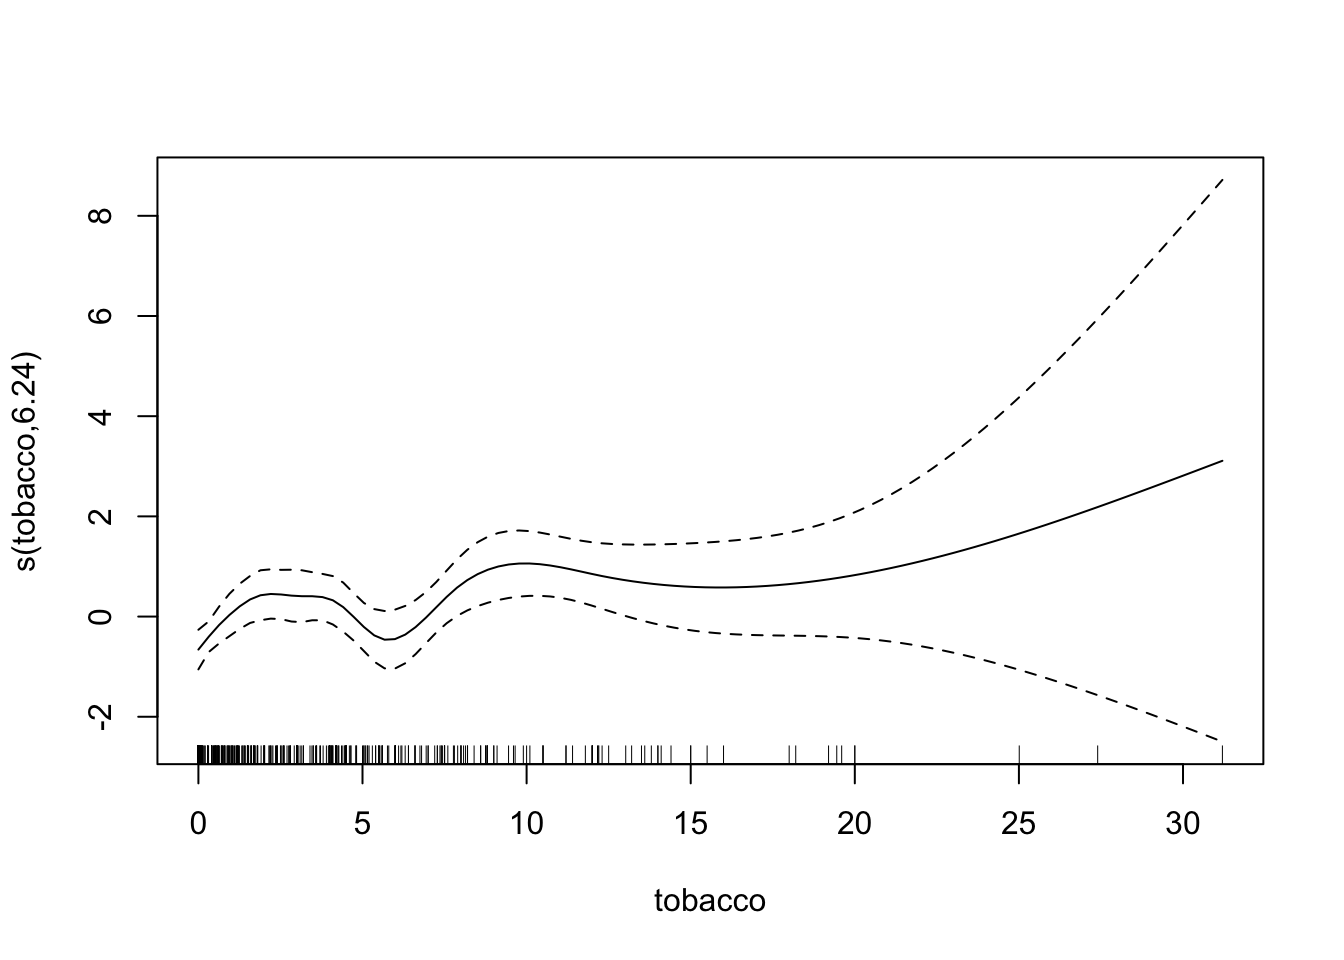
\includegraphics[keepaspectratio]{_main_files/figure-latex/unnamed-chunk-22-1.pdf}} \pandocbounded{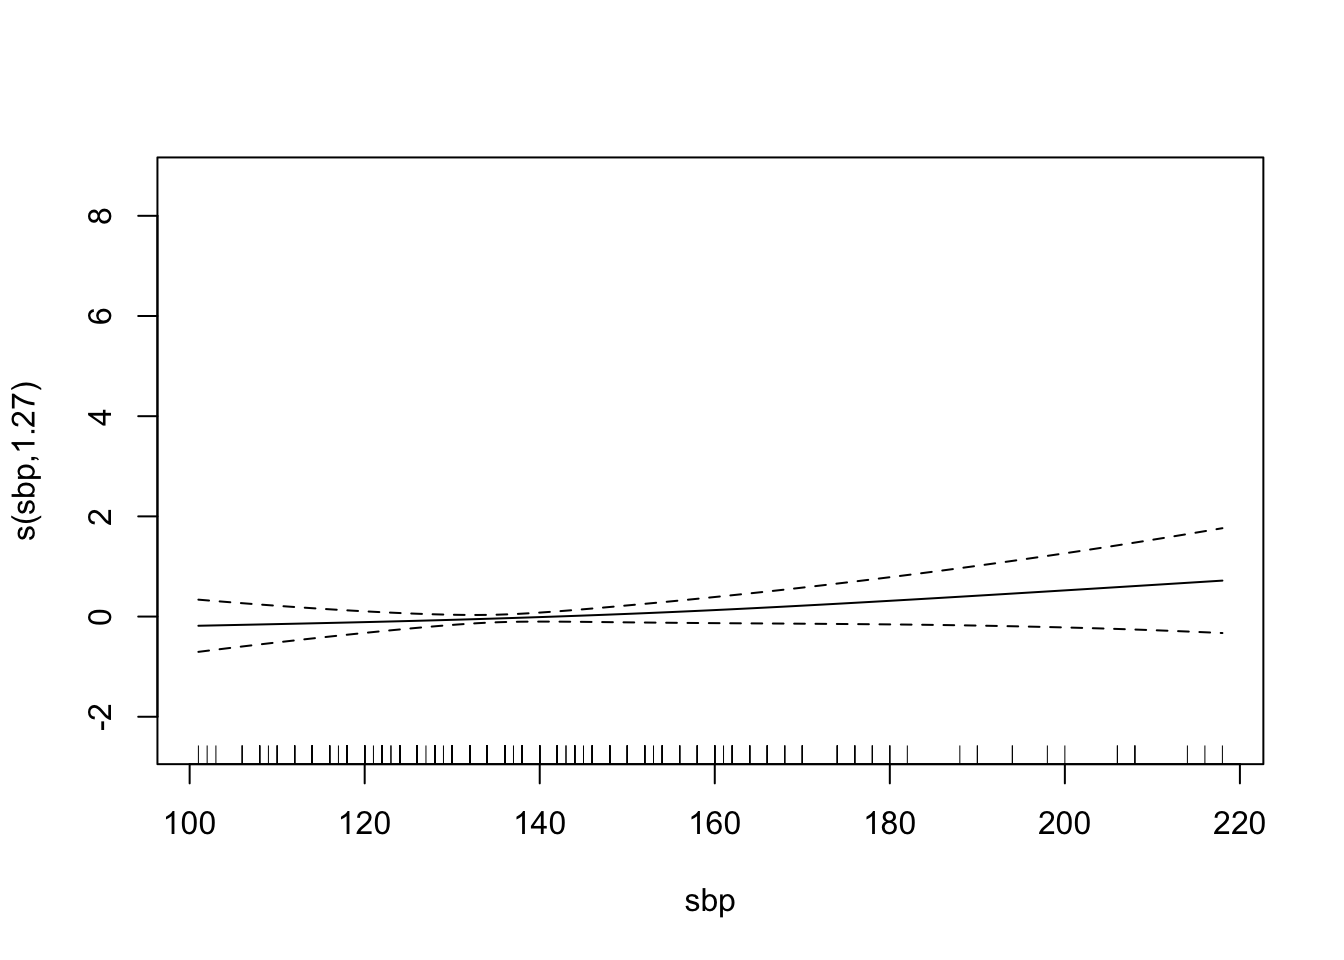
\includegraphics[keepaspectratio]{_main_files/figure-latex/unnamed-chunk-22-2.pdf}} \pandocbounded{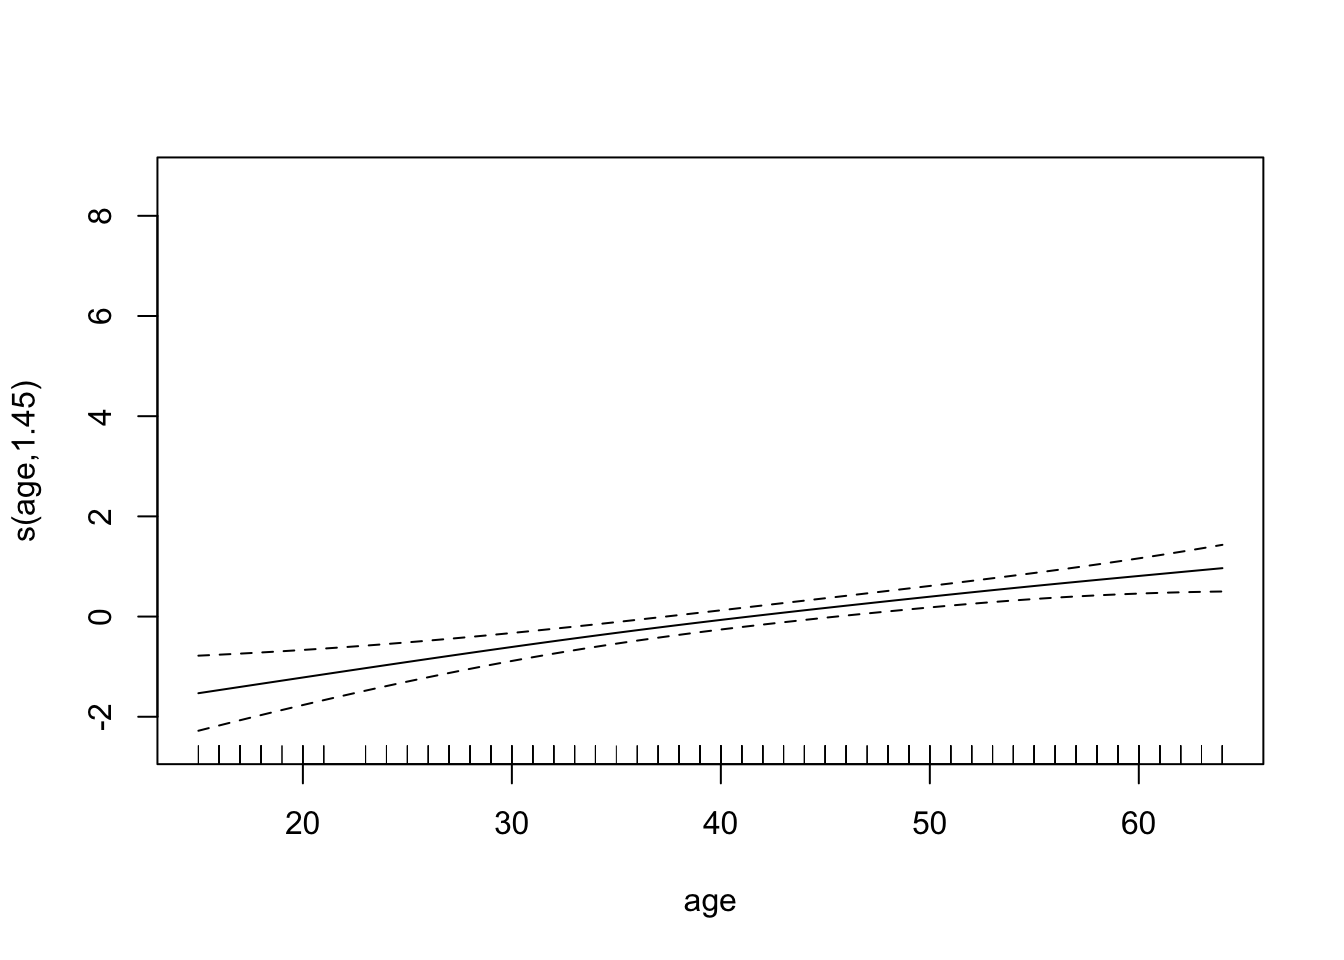
\includegraphics[keepaspectratio]{_main_files/figure-latex/unnamed-chunk-22-3.pdf}}

\begin{enumerate}
\def\labelenumi{\alph{enumi})}
\setcounter{enumi}{1}
\item
  Find the AUC ROC for the model above.
\item
  Compare the AUC ROC of the GAM model with a logistic regression with
  linear effects for the predictors.
\end{enumerate}

\begin{enumerate}
\def\labelenumi{\arabic{enumi})}
\setcounter{enumi}{1}
\tightlist
\item
  The dataset \href{https://www.dropbox.com/s/jeqdtq04zl9f0er/FEV.csv?dl=1}{fev.csv} contains the measurements of forced expiratory volume (FEV) tests, evaluating the pulmonary capacity in 654 children and young adults.
\end{enumerate}

\begin{enumerate}
\def\labelenumi{\alph{enumi})}
\item
  Plot the association between \emph{fev} and \emph{height} and fit a smoothing spline for \emph{fev} using \emph{height} as a predictor
\item
  Plot the association between \emph{fev} and \emph{age} and fit a smoothing spline for \emph{fev} using \emph{age} as a predictor
\item
  Fit a GAM model for \emph{fev} with smoothing slipes for \emph{height} and \emph{age} and also add \emph{sex} to the model.
\item
  Comment in the results of the fitted GAM model and plot the fitted splines for the predictors
\end{enumerate}

\end{document}
